\documentclass{ieeeaccess}
\usepackage{cite}
\usepackage{amsmath,amssymb,amsfonts}
\usepackage{algorithmic}
\usepackage{algorithm}
\usepackage{graphicx}
\usepackage{adjustbox}
\usepackage{url}
\usepackage{array}
\usepackage{textcomp}
\def\BibTeX{{\rm B\kern-.05em{\sc i\kern-.025em b}\kern-.08em
    T\kern-.1667em\lower.7ex\hbox{E}\kern-.125emX}}
\begin{document}
\history{Manuscript under review, November 2026.}

\title{Performance Evaluation of a Compiler's Symbol Table Implementation: Collision Resolution Strategies}

\author{\uppercase{Syed Ayman Alam}\authorrefmark{1},
\uppercase{Girijeshvasan M}\authorrefmark{1}, and
\uppercase{Brajesh Agrawal}\authorrefmark{1}}
\address[1]{School of Computer Science and Engineering (SCOPE), Vellore Institute of Technology, Vellore, Tamil Nadu, India (e-mail: syed.aymanalam2024@vitstudents.ac.in; girijeshvasan.m2024@vitstudent.ac.in; brajesh.kumar2024@vitstudent.ac.in)}

\markboth
{Alam \headeretal: Performance Evaluation of a Compiler's Symbol Table Implementation}
{Alam \headeretal: Performance Evaluation of a Compiler's Symbol Table Implementation}

\corresp{Corresponding author: Syed Ayman Alam (e-mail: syed.aymanalam2024@vitstudents.ac.in).}

\begin{abstract}
Symbol tables are central compiler data structures that map identifiers to type, scope and storage information, and their lookup cost affects every compiler phase. We implemented eight collision-resolution designs in one C++17 library (separate chaining, linear probing, quadratic probing, double hashing, Robin Hood hashing and three hybrids: H1 chaining with red-black-tree buckets, H2 bounded probing with an overflow chain, H3 bucketized cuckoo hashing with a stash) together with five string hash functions and two block-scope designs. In a fixed-capacity experiment (10,007 slots, load factors 0.1--0.95, 30 trials, two hash functions) we report means, standard deviations and 95 \% confidence intervals using a probe metric that counts memory locations consistently across strategies. At load factor 0.9 an unsuccessful search costs 53.2 probes with linear probing (theory 50.5), 6.0 with Robin Hood hashing, 5.4 with H2 and 1.9 with separate chaining. Robin Hood hashing leaves the mean successful-search cost of linear probing unchanged (5.49) but cuts its variance from 293 to 23. Stress tests with weak-hash and multi-collision keys show when each hybrid mechanism fires: H1 cut the successful-search cost on 4,096 colliding keys from 2050 to 14 probes. A resizing experiment over seven workloads, including identifier streams captured from the Lua, zlib, Redis and SQLite sources, and a comparison of the name@depth scope design with a conventional shadow-chain design (2.6--3.2$\times$ faster at nesting depth 8) complete the study. Results support choosing a strategy from the workload and hash function rather than a universal ranking.
\end{abstract}

\begin{keywords}
Collision resolution, Compiler, Hash function, Performance evaluation, Scope management, Symbol table, Workload
\end{keywords}

\titlepgskip=-15pt

\maketitle

\section{Introduction}

A compiler symbol table records the attributes of every identifier and makes them available during parsing, semantic analysis, type checking, scope resolution and code generation. It must support insertion, lookup, deletion or scope exit, and queries that depend on the currently visible declaration. Hash tables are the usual choice because their expected cost is close to constant, but collisions, high load factors, key distributions, deletion policies and memory layout change the observed cost substantially [1]--[3]. Compiler textbooks describe hashing for symbol tables [4], [5], yet they rarely compare collision-resolution strategies under one measurement protocol.

We address a narrow, practical question: how do different collision-resolution strategies behave when they are implemented in one C++17 library and measured with the same keys, the same probe definition and the same harness, on random identifiers, adversarial identifiers, and identifiers taken from real compiler workloads? We compare separate chaining, linear, quadratic and double hashing, Robin Hood hashing [6] and three hybrids that we designed to bound the worst case of chaining, of open addressing and of cuckoo hashing [7], [8].

Our contributions are: (i) a library of eight strategies, five hash functions and two block-scope designs behind one interface; (ii) a probe metric that counts memory locations consistently, so that chaining and open addressing can be compared directly; (iii) a fixed-capacity study with 30 trials per point, two hash functions, confidence intervals and a validation against the classical linear-probing formulas; (iv) stress tests that show when the hybrid mechanisms (tree conversion, overflow chain, stash) are actually used; (v) a resizing study over synthetic workloads and identifier streams captured from four open-source C code bases; and (vi) a specification and evaluation of the scope-handling design against a conventional shadow-chain design.

Section II reviews recent work and states the research gap. Section III defines the system, the metrics, the probe counting and the scope designs. Section IV describes the environment and the experiments, Section V reports results, and Sections VI--VIII cover verification, limitations and conclusions. Declarations on author contributions, the use of AI tools, and data and code availability close the paper.

\section{Related Work}

\subsection{Open Addressing and Primary Clustering}

Knuth's analysis gives the expected successful and unsuccessful search costs of linear probing [1], and the same analysis explains why linear probing is avoided at high load. Bender \emph{et al.} showed that deletion design changes this picture: tombstones can act against primary clustering, and a ``graveyard'' variant keeps insertion cost low at any sequence of operations [9]; Chesetti \emph{et al.} later removed the periodic stop-the-world redistribution this needs [10]. Farach-Colton \emph{et al.} proved tight probe bounds for open addressing without reordering and disproved a long-standing conjecture on uniform probing [11]. These works concern asymptotics and integer keys; our study measures what happens at fixed load for string identifiers.

\subsection{Cuckoo Hashing, Stashes and Bucketized Designs}

Cuckoo hashing [7] bounds lookups to a few candidate locations; adding a small stash makes insertion failures rare [8], which is the mechanism of our H3. Li \emph{et al.} engineered concurrent cuckoo tables [12], Breslow \emph{et al.} reduced the number of cache lines touched by bucketized cuckoo lookups [13], and Bender \emph{et al.} combined front-yard/back-yard layout with low associativity and stability in Iceberg hashing [14]. Maier \emph{et al.} benchmarked concurrent tables against widely used libraries [15]. All of these target integer or fixed-size keys and general-purpose workloads, not the scoped, string-keyed, delete-heavy pattern of a symbol table.

\subsection{Comparative Evaluation and Hash Functions}

Richter \emph{et al.} compared chaining, linear, quadratic, cuckoo and Robin Hood hashing along seven dimensions and showed that the best scheme depends on load factor, key distribution, read/write ratio and hash function [3]. Ramakrishna and Zobel studied string hash functions in practice [16], Thorup surveyed tabulation hashing with strong guarantees [17], and Sabek \emph{et al.} found that learned models can replace hash functions only for suitable distributions [18], [19]. Aumasson and Bernstein motivated keyed hashing by hash-flooding attacks [20], which is the threat our multi-collision stress test models.

\subsection{String-Keyed Structures and Symbol Management}

Askitis and Sinha combined tries with hash buckets for cache-efficient string storage [21]. Moreno \emph{et al.} replaced the lock-based atom (symbol) table of a Prolog system with a lock-free hash trie to scale symbol management across threads [22]. Symbol-table design in compilers is otherwise treated as textbook material [4], [5].

\begin{table}[!t]
\caption{Summary of the related work reviewed in Section II.}
\label{tab:1}
\centering
\scriptsize
\setlength{\tabcolsep}{3pt}
\begin{tabular}{|>{\raggedright\arraybackslash}p{0.113\columnwidth}|>{\raggedright\arraybackslash}p{0.183\columnwidth}|>{\raggedright\arraybackslash}p{0.306\columnwidth}|>{\raggedright\arraybackslash}p{0.278\columnwidth}|}
\hline
\textbf{Ref.} & \textbf{Year / venue} & \textbf{Contribution} & \textbf{Relation to this study} \\
\hline
{}[1] & 1998, book & Classical analysis of probing and chaining & Baseline formulas validated in Table 9 \\
{}[8] & 2009, SICOMP & Cuckoo hashing with a constant-size stash & Mechanism of H3; we measure when the stash is used \\
{}[21] & 2010, VLDB J. & HAT-trie: cache-conscious string keys & Alternative string-key structure; not covered here \\
{}[20] & 2012, INDOCRYPT & Keyed hash function against hash flooding & Motivates the multi-collision stress test \\
{}[12] & 2014, EuroSys & Fast concurrent optimistic cuckoo hashing & Single-threaded here; concurrency is future work \\
{}[3] & 2015, PVLDB & Seven-dimension comparison of hashing schemes & Closest in method; integer keys, no scopes or compiler data \\
{}[13] & 2016, USENIX ATC & Horton tables: fewer buckets per lookup & Related to H3 miss cost (always 8 slots) \\
{}[17] & 2017, CACM & Tabulation hashing with strong guarantees & Stronger hash functions than the five tested \\
{}[19] & 2018, SIGMOD & Learned index structures & Learned alternatives to hashing, not evaluated \\
{}[15] & 2019, TOPC & Concurrent hash tables, extensive comparison & Concurrency; word-sized keys \\
{}[9] & 2021, FOCS & Tombstones defeat primary clustering & Explains linear-probing behaviour under deletes \\
{}[18] & 2022, PVLDB & Learned models as hash functions & Hash function choice matters; our weak hash shows extreme case \\
{}[14] & 2023, JACM & Iceberg hashing: stable, space-efficient & Design space beyond our eight strategies \\
{}[11] & 2024, FOCS & Optimal open addressing without reordering & Theory for the open-addressing family \\
{}[22] & 2024, IJPP & Lock-free atom table for Prolog symbols & Only symbol-table paper in the set; concurrency focus \\
{}[10] & 2025, SIGMOD & Zombie hashing: deamortized tombstones & Deletion handling for linear probing \\
\hline
\end{tabular}
\end{table}


\subsection{Research Gap}

The works above establish algorithms, bounds and engineering for hash tables with integer or fixed-size keys. None of them compares collision-resolution strategies for compiler symbol tables under one probe definition, with adversarial and real-code identifier streams, resizing, deletion and block-scope operations. The only symbol-table paper we found targets concurrency [22]. We therefore contribute a controlled, reproducible, single-threaded comparison that includes the scope-handling design, and we state clearly that its results hold for this implementation and these workloads.

\section{System Design}

\subsection{Problem Formulation}

A symbol table stores identifier records under a chosen hash function and collision-resolution strategy. For every operation it must keep dictionary semantics: inserted keys are retrievable, absent keys are not returned, and deleted keys disappear. Our objective is to compare operation costs while the functional behaviour stays identical, using probe counts, elapsed time, failed insertions and memory.

A compiler adds block structure: a name declared in an outer block is hidden by a declaration of the same name in an inner block, and leaving a block must remove the inner declarations. Sections III-E and V-E specify and evaluate two designs for this.

\begin{figure*}[!t]
\centering
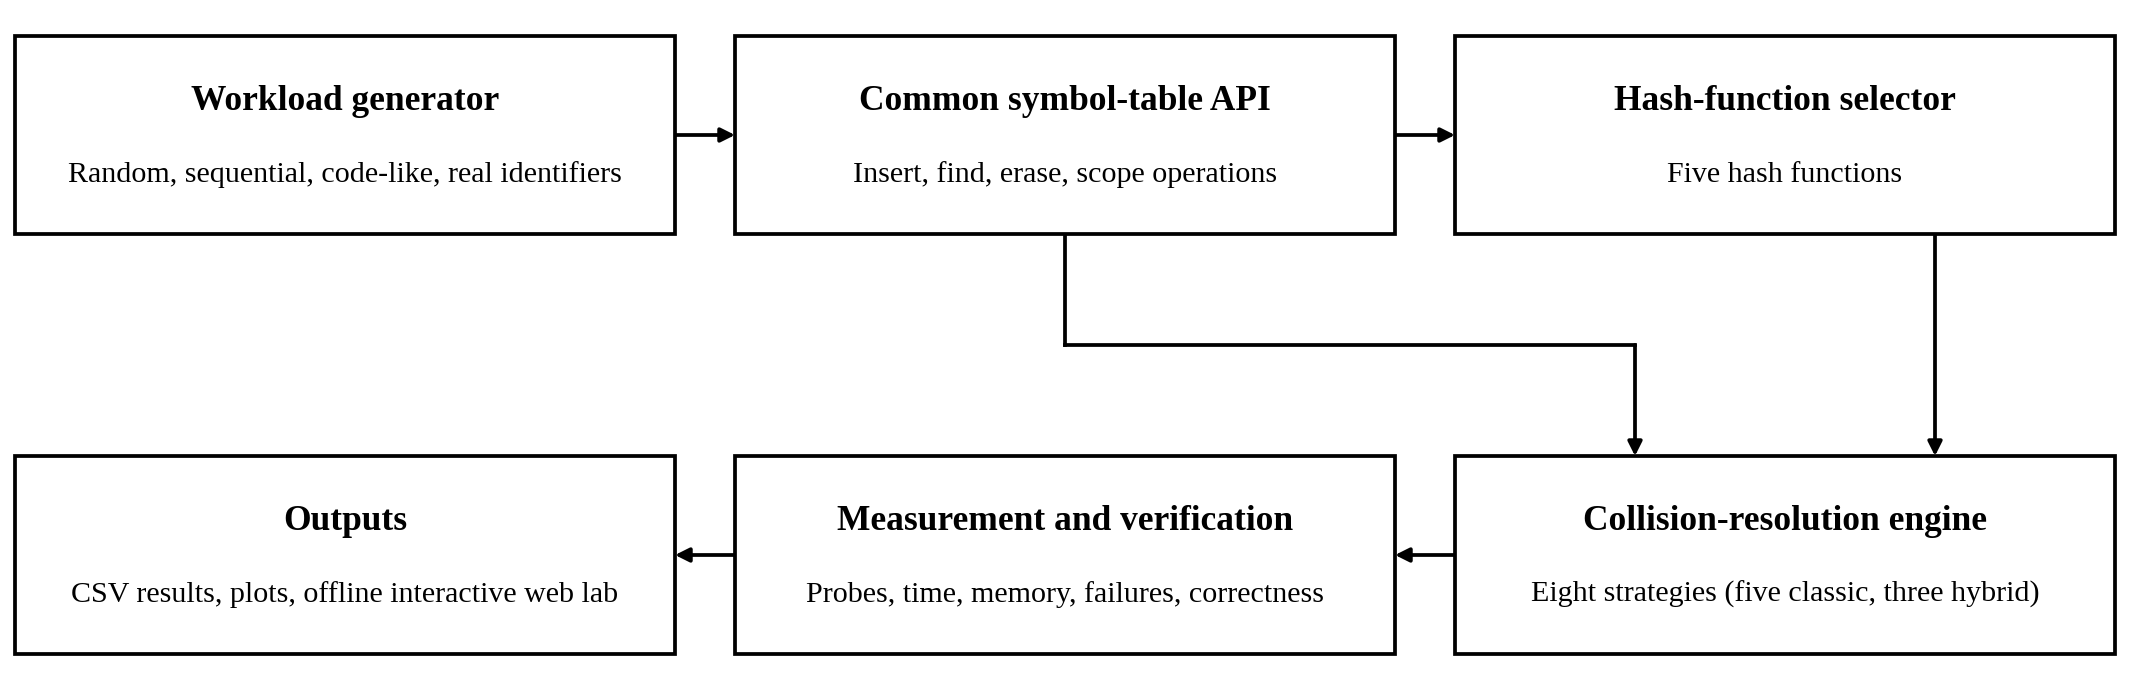
\includegraphics[width=0.92\textwidth]{fig1.png}
\caption{Architecture of the evaluation framework.}
\label{fig:1}
\end{figure*}

Fig. 1 shows the path from workload generation through the common interface, hash selection and collision strategy to the metrics and CSV outputs. The browser lab (lab/) offers a second interface to the same operations: a visualizer of probe traces, a configurable benchmark, a compiler mode that replays source code, a hash-distribution lab and in-browser tests. A JavaScript engine reproduces the C++ engine, and the two agree on probes, collisions, resizes, failures and memory estimates for identical operation scripts (Section VI). A front end of this kind couples parsing with symbol-table lookups [4]; modern production tables such as Swiss tables and F14 use metadata and group probing [23], [24].

\subsection{Implemented Strategies}

Table 2 lists the eight strategies. The three hybrids are our own designs and expose counters for their special mechanisms (tree conversions, overflow spills, stash placements), which Sections V-D and V-F use.

\begin{table}[!t]
\caption{Implemented collision-resolution strategies.}
\label{tab:2}
\centering
\scriptsize
\setlength{\tabcolsep}{3pt}
\begin{tabular}{|>{\raggedright\arraybackslash}p{0.201\columnwidth}|>{\raggedright\arraybackslash}p{0.358\columnwidth}|>{\raggedright\arraybackslash}p{0.321\columnwidth}|}
\hline
\textbf{Strategy} & \textbf{Behaviour} & \textbf{Expected trade-off} \\
\hline
Separate chaining & Each bucket owns a linked list of entries. & Miss cost follows bucket occupancy; pointer and allocation overhead. \\
Linear probing & Checks consecutive slots until match or empty slot. & Locality, but primary clustering raises miss and tail cost. \\
Quadratic probing & Probe offsets i\textsuperscript{2}. & Less clustering; may not reach every slot. \\
Double hashing & Second hash sets the step. & Disperses probe sequences better than linear probing. \\
Robin Hood hashing & Insertion swaps with residents closer to home; lookup stops early. & Lower variance of probe length; relocation work on insert. \\
H1: chaining + tree & A chain longer than 8 becomes a red-black tree; reverts at 4. & Bounds chain search at O(log n); tree nodes cost memory. \\
H2: bounded probing + overflow & Probe an 8-slot window; a key that does not fit goes to an overflow chain. & Bounded slot scans; overflow chain and pointers. \\
H3: bucketized cuckoo + stash & Two hashes, 4-slot buckets, 4-entry stash, at most 200 kicks. & At most two buckets per lookup; displacement chains on insert. \\
\hline
\end{tabular}
\end{table}


\subsection{Hash Functions}

Five hash functions are supported: djb2, 64-bit FNV-1a, sdbm, PJW (ELF), and a deliberately weak sum of characters. The weak function is a stress case, not a recommendation: anagrams and many differently ordered names collide. Experiment A uses djb2 for the headline results and repeats the sweep with FNV-1a; Experiment B uses all five.

\subsection{Metrics, Probe Counting and Mathematical Definitions}

Let n be the number of stored entries, m the number of slots (or buckets) and $\alpha$ the load factor. For q measured operations, let p\textsubscript{i} be the probes of operation i and t\textsubscript{i} its elapsed time. The metrics are

\begin{equation}
\alpha = \frac{n}{m}
\end{equation}

\begin{equation}
\bar{P} = \frac{1}{q}\sum_{i=1}^{q} p_i
\end{equation}

\begin{equation}
\bar{T} = \frac{1}{q}\sum_{i=1}^{q} t_i
\end{equation}

\begin{equation}
P_{\max} = \max_{i=1,\ldots,q} p_i
\end{equation}

\begin{equation}
\text{Failure rate} = \frac{\text{failed insertions}}{\text{attempted insertions}}
\end{equation}

\begin{equation}
\text{Bytes per entry} = \frac{\text{estimated table bytes}}{\text{stored entries}}
\end{equation}

\begin{equation}
\text{Scope cost} = \frac{\text{scope-operation time}}{\text{number of scope operations}}
\end{equation}

\begin{equation}
P_{hit} \approx \frac{1}{2}\left[1+\frac{1}{1-\alpha}\right]
\end{equation}

\begin{equation}
P_{miss} \approx \frac{1}{2}\left[1+\frac{1}{(1-\alpha)^{2}}\right]
\end{equation}

where P\textsubscript{hit} in (8) and P\textsubscript{miss} in (9) are Knuth's expected numbers of probes for a successful and an unsuccessful search under linear probing [1]. Eq. (8) is the successful-search formula and (9) the unsuccessful-search formula; in an earlier version of this work (8) was used for both, which is wrong for unsuccessful searches. P\textsubscript{max} in (4) is the maximum over the q operations. In (7) a scope operation is one declaration, one resolve, or one erase performed when a scope exits.

\textbf{Probe definition.} A probe is one distinct memory location whose key or state is examined: a table slot, a bucket-head pointer, a list node, or a tree level. The raw counter of the library does not count the bucket-head read of chaining and H1 lookups, so an empty bucket costs 0 probes; open addressing counts the empty slot it stops at. This would make the comparison of 0.9 against 53 probes at $\alpha$ = 0.9 partly an artefact. We therefore report a \emph{consistent} probe metric, equal to the raw counter plus one for lookups in chaining and H1, and give the raw value where it matters. Insertion counters already agree: a chaining insert counts one bucket-head read plus the nodes scanned, which equals the raw value (nodes scanned plus one). H1 tree buckets use the estimate $\lceil$log\textsubscript{2}(size + 1)$\rceil$ per access, not a count of real comparisons. A probe remains a logical unit: a list node, a slot and a tree level do not have equal latency, so we report timing separately.

\begin{table}[!t]
\caption{Probe definition per strategy.}
\label{tab:3}
\centering
\scriptsize
\setlength{\tabcolsep}{3pt}
\begin{tabular}{|>{\raggedright\arraybackslash}p{0.218\columnwidth}|>{\raggedright\arraybackslash}p{0.487\columnwidth}|>{\raggedright\arraybackslash}p{0.175\columnwidth}|}
\hline
\textbf{Strategy} & \textbf{One probe is \ldots{}} & \textbf{Consistent vs. raw} \\
\hline
Chaining & one list node (raw); consistent also counts the bucket-head read & +1 on lookups \\
Linear / quadratic / double & one table slot, including the empty slot that ends a search & equal \\
Robin Hood & one slot; a lookup stops when the resident is closer to home & equal \\
H1 & one list node, or $\lceil$log\textsubscript{2}(size+1)$\rceil$ levels for a tree bucket; plus bucket head & +1 on lookups \\
H2 & one slot of the 8-slot window, or one overflow node & equal \\
H3 & one slot of either candidate bucket, or one stash entry & equal \\
\hline
\end{tabular}
\end{table}


\subsection{Scope-Handling Designs}

The original design, \emph{name@depth}, mangles every declaration into the key name@d, where d is the current lexical depth, and inserts it into the table. Algorithm 2 gives the lookup procedure that earlier versions left undefined. Its cost is one table lookup per candidate depth, each preceded by a string concatenation, so a successful resolve costs (current depth $-$ declaring depth + 1) lookups and an unsuccessful resolve costs (current depth + 1) lookups.

\begin{algorithm}[!t]
\caption{Benchmark one strategy}
\begin{algorithmic}[1]
\STATE Select the strategy, hash function, capacity and workload.
\STATE Construct the table and insert the common key set in the specified order.
\STATE For each operation record the probe count and the elapsed time.
\STATE Verify that every stored key is found and every absent key stays absent.
\STATE Verify that deleted keys are gone; record failures and the memory estimate.
\STATE Repeat for the prescribed trials; export one CSV row per trial.
\end{algorithmic}
\end{algorithm}

\begin{algorithm}[!t]
\caption{Block scopes with name@depth keys}
\begin{algorithmic}[1]
\STATE enter\_scope: push an empty list of declared keys; depth $\leftarrow$ depth + 1.
\STATE declare(x): k $\leftarrow$ x + ``@'' + depth; insert k; append k to the current list.
\STATE resolve(x): for d $\leftarrow$ depth down to 0: k $\leftarrow$ x + ``@'' + d; if lookup(k) succeeds, return it. Return ``not found''.
\STATE exit\_scope: erase every key of the current list; pop the list; depth $\leftarrow$ depth $-$ 1.
\end{algorithmic}
\end{algorithm}

The conventional alternative, the \emph{shadow chain}, keeps one table entry per plain name holding the innermost visible declaration; each declaration remembers the one it shadows. Algorithm 3 shows it. Resolve is one table lookup regardless of depth and needs no concatenation; declare costs one lookup and one insert; exit\_scope restores or erases one entry per declaration. We implemented both on top of every strategy and compare them in Section V-E.

\begin{algorithm}[!t]
\caption{Block scopes with shadow chains}
\begin{algorithmic}[1]
\STATE enter\_scope: remember the current size of the declaration stack.
\STATE declare(x): look up x; if its entry belongs to the current depth, update it in place; otherwise push (declaration, shadowed entry) on the stack and insert or overwrite the entry for x.
\STATE resolve(x): return lookup(x).
\STATE exit\_scope: pop declarations down to the remembered size; for each one restore the shadowed declaration (insert) or erase x if nothing was shadowed.
\end{algorithmic}
\end{algorithm}

\subsection{Operation Flow and Modules}

\begin{figure}[!t]
\centering
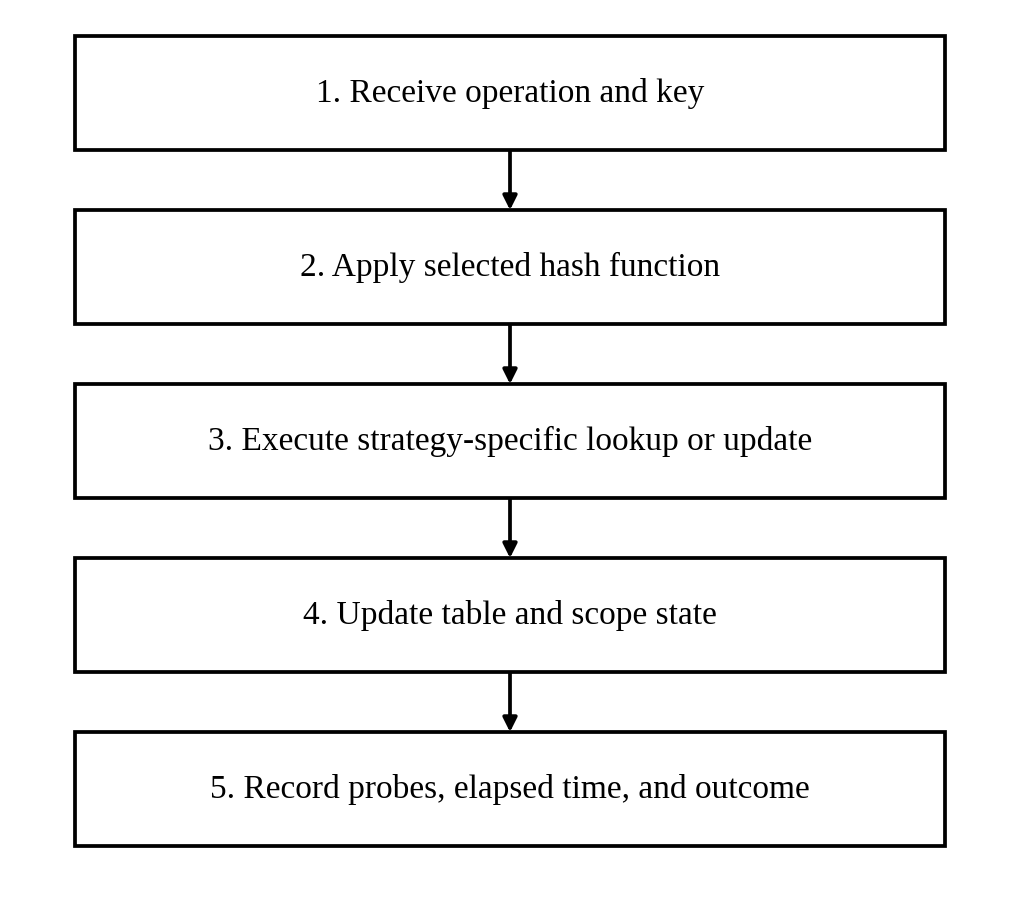
\includegraphics[width=\columnwidth]{fig2.png}
\caption{General operation and measurement flow.}
\label{fig:2}
\end{figure}

\begin{table}[!t]
\caption{Software modules.}
\label{tab:4}
\centering
\scriptsize
\setlength{\tabcolsep}{3pt}
\begin{tabular}{|>{\raggedright\arraybackslash}p{0.262\columnwidth}|>{\raggedright\arraybackslash}p{0.618\columnwidth}|}
\hline
\textbf{Module} & \textbf{Responsibility} \\
\hline
symtab.h / symtab.cpp & Strategies, hash functions, hybrid counters, both scope managers. \\
benchmark.cpp & Original load-factor sweep and extended workloads. \\
experiments.cpp & Per-trial sweeps, probe-length distributions, hybrid stress tests, scope designs, Experiment B, real-code traces. \\
test\_correctness.cpp & Hash vectors, edge cases, scopes, differential fuzzing. \\
symtab\_cli.cpp & Scripted operations for the JavaScript cross-check. \\
lab/ & Offline browser lab: visualizer, benchmark, compiler replay, hash lab, tests. \\
analysis/analyze.py & Statistics, figures and tables from the raw CSV files. \\
\hline
\end{tabular}
\end{table}


\section{Experimental Setup}

\subsection{Environment}

All measurements reported in this paper were taken in one session on one machine, whose full configuration is given in Table 5. It is a virtualized single-core server, so absolute timings are specific to it and are noisy; we therefore repeat every timed point and report dispersion, and we interpret probe counts, which do not depend on the machine, separately from times. The code was compiled with -O2.

\begin{table}[!t]
\caption{Hardware and software environment of all measurements.}
\label{tab:5}
\centering
\scriptsize
\setlength{\tabcolsep}{3pt}
\begin{tabular}{|>{\raggedright\arraybackslash}p{0.218\columnwidth}|>{\raggedright\arraybackslash}p{0.662\columnwidth}|}
\hline
\textbf{Item} & \textbf{Value} \\
\hline
CPU & Intel Xeon Processor (virtualized), 2.10 GHz, 1 vCPU \\
Memory & 3.9 GiB RAM \\
Operating system & Ubuntu 24.04.4 LTS, x86-64 \\
C++ compiler & g++ (Ubuntu 13.3.0-6ubuntu2\textasciitilde{}24.04.1) 13.3.0 \\
Build flags & -O2 -std=c++17 -Wall -Wextra (tests: -O1 -g -fsanitize=address,undefined) \\
Timer / allocator & std::chrono::steady\_clock; glibc malloc (heap measured with mallinfo2) \\
Analysis software & Python 3.12.3; pandas, matplotlib, SciPy, NumPy 3.0.2 3.10.8 1.17.1 2.4.4; Node.js v22.22.2 \\
Real source code & Lua 5.4.7, zlib 1.3.1, Redis 7.2.5, SQLite 3.46.0 (release tags) \\
\hline
\end{tabular}
\end{table}


\subsection{Workloads}

\textbf{Synthetic.} \emph{Random} identifiers have 3--15 characters, start with a letter and use letters, digits and underscore. \emph{Sequential} identifiers are var0, var1, \ldots{}. \emph{Code-like} identifiers combine 24 common programming words, optional suffix numbers and an m\_ prefix. \textbf{Real code.} We extracted identifiers from all C files of four open-source projects, [25], [26], [27] (src/) and [28] (src/), with comments, string literals, preprocessor lines and C keywords removed. Table 6 describes them. The \emph{-ids} workloads in Experiment B are the sets of unique identifiers per project. The \emph{traces} of Section V-G replay every identifier token in source order, one table per source file, as a lexer with an interning symbol table would: a token is looked up and inserted if absent. A \emph{scoped} replay additionally issues enter/exit\_scope at braces and declarations for identifiers that follow a type keyword or type name; this declaration heuristic has no full parser behind it.

\begin{table*}[!t]
\caption{Real-code workloads (identifier counts after removing comments, strings, directives and keywords).}
\label{tab:6}
\centering
\scriptsize
\adjustbox{max width=\textwidth}{%
\begin{tabular}{|l|l|l|l|l|l|l|l|l|l|}
\hline
\textbf{Corpus} & \textbf{Files} & \textbf{Source lines} & \textbf{Id. tokens} & \textbf{Unique ids} & \textbf{Unique / file (mean)} & \textbf{Unique / file (max)} & \textbf{Decl. events} & \textbf{Use events} & \textbf{Max depth} \\
\hline
lua & 35 & 26,044 & 43,445 & 3,351 & 201 & 589 & 6,466 & 37,321 & 8 \\
zlib & 15 & 9,539 & 13,897 & 878 & 103 & 297 & 1,109 & 12,850 & 9 \\
redis & 102 & 136,374 & 210,029 & 12,833 & 260 & 2,636 & 23,580 & 186,083 & 9 \\
sqlite & 128 & 202,251 & 280,332 & 13,835 & 268 & 1,243 & 30,635 & 250,326 & 10 \\
\hline
\end{tabular}}
\end{table*}


\subsection{Experiments and Statistics}

\textbf{Experiment A} uses a fixed capacity of 10,007 slots (cuckoo: 10,012), twelve load factors from 0.1 to 0.95, and n = $\lfloor$10,007 $\alpha$$\rfloor$ random keys that are identical for every strategy. Each point is repeated for 30 trials with different keys. For each trial we insert n keys, search the n keys (five passes, mean per pass) and search n absent keys of the same kind. The main comparison uses \textbf{djb2}, the default hash function of the library; we repeat it with \textbf{FNV-1a}. We report mean $\pm$ standard deviation over trials and, for plots, 95 \% confidence intervals from the t distribution with 29 degrees of freedom. \textbf{Experiment B} starts with 1,031 slots and resizes at maximum load 0.7; it covers seven workloads, five hash functions, eight strategies, insert, hit, miss and delete phases and the block-scope workload of Section III-E. Every cell is repeated 5 times (three times for the weak sum hash, whose clustered cases cost O(n\textsuperscript{2}) and were limited to 10,000 keys) and reported as the median. Run-to-run SD of a median is 7 \% of the value in a typical cell, so differences below about 15 \% should not be read as ranking evidence.

\begin{table}[!t]
\caption{Experimental parameters.}
\label{tab:7}
\centering
\scriptsize
\setlength{\tabcolsep}{3pt}
\begin{tabular}{|>{\raggedright\arraybackslash}p{0.157\columnwidth}|>{\raggedright\arraybackslash}p{0.175\columnwidth}|>{\raggedright\arraybackslash}p{0.297\columnwidth}|>{\raggedright\arraybackslash}p{0.251\columnwidth}|}
\hline
\textbf{Parameter} & \textbf{Experiment A} & \textbf{Experiment B} & \textbf{Traces} \\
\hline
Capacity & 10,007 fixed & 1,031, grows at $\alpha$ > 0.7 & 211, grows at $\alpha$ > 0.7 \\
Keys & random, 3--15 chars & random, sequential, code-like; four real unique-id sets & identifier tokens of C files \\
Repetitions & 30 trials & 5 (3 for sum hash) & 3 \\
Hash & djb2; FNV-1a & all five & djb2; FNV-1a \\
Operations & insert, hit, miss & insert, hit, miss, delete, scope & lookup+insert; scoped replay \\
Reported & mean $\pm$ SD, 95 \% CI & median & median \\
\hline
\end{tabular}
\end{table}


\section{Results}

\subsection{Experiment A: Fixed-Capacity Sweep}

\begin{figure*}[!t]
\centering
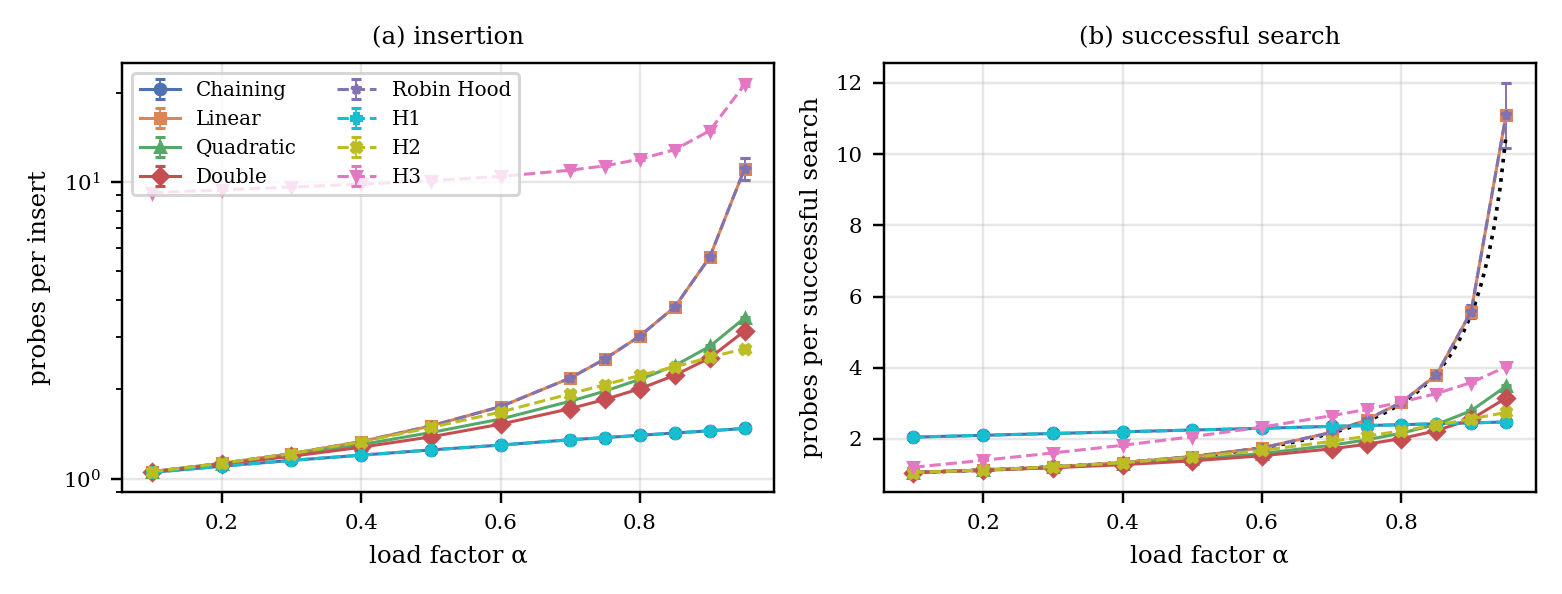
\includegraphics[width=0.92\textwidth]{fig3.png}
\caption{Insertion and successful-search probes versus load factor (djb2, mean over 30 trials, bars: 95 \% CI; dotted: Eq. (8)).}
\label{fig:3}
\end{figure*}

Insertion probes rise with load for every strategy (Fig. 3a). At $\alpha$ = 0.9 chaining and H1 need 1.45 probes, H2 2.56, double hashing 2.55, quadratic probing 2.79, linear probing and Robin Hood hashing 5.58, and H3 14.87 because cuckoo kicks and slot scans are counted. Successful search (Fig. 3b) follows Eq. (8) for linear probing within the confidence interval (5.58 $\pm$ 0.17 against 5.50 at $\alpha$ = 0.9). Linear probing and Robin Hood hashing have \emph{identical} mean costs in Fig. 3 and Fig. 4a. This is expected: Robin Hood hashing moves entries so that probe lengths equalize, but the sum of the displacements of all keys is unchanged, so the mean successful-search cost cannot change; the benefit appears in the distribution (Section V-B).

\begin{figure*}[!t]
\centering
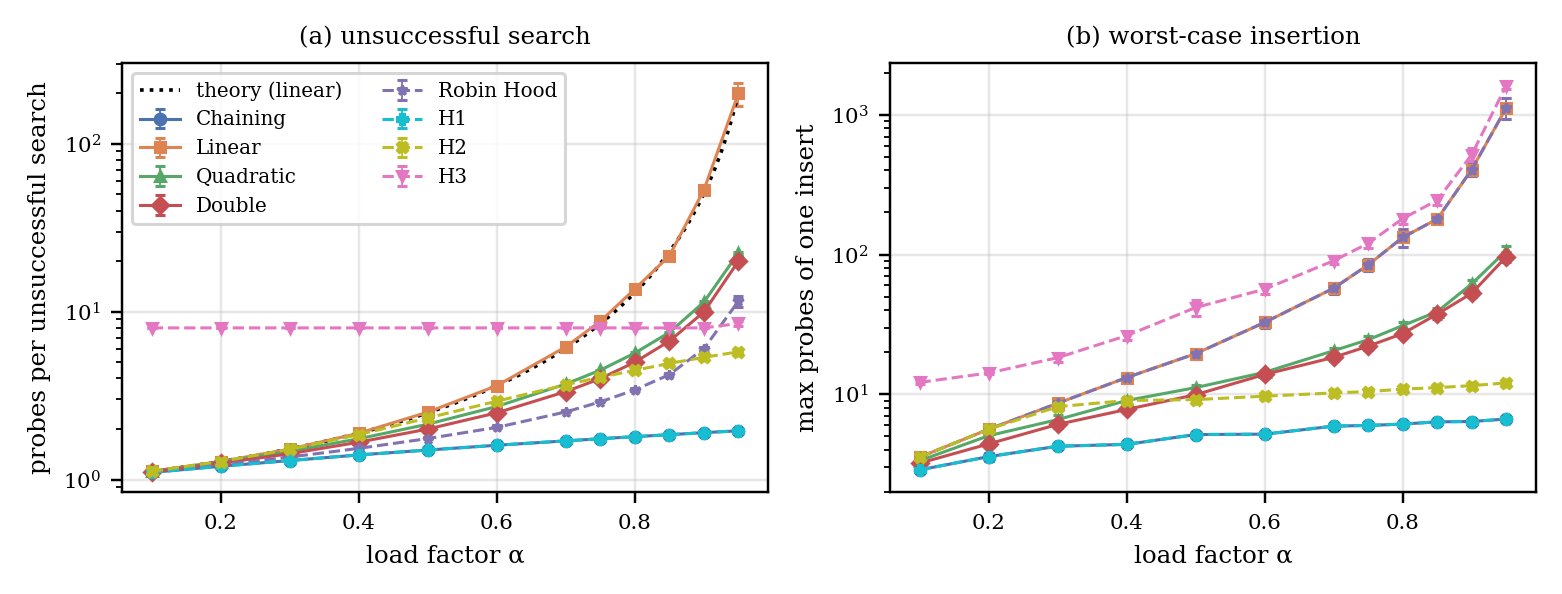
\includegraphics[width=0.92\textwidth]{fig4.png}
\caption{Unsuccessful-search probes (consistent metric; dotted: Eq. (9)) and worst-case insertion probes (median over trials) versus load factor.}
\label{fig:4}
\end{figure*}

Unsuccessful search (Fig. 4a, Table 8) is the most sensitive metric. At $\alpha$ = 0.9 linear probing needs 53.15 $\pm$ 3.94 probes (95 \% CI) against 50.50 from Eq. (9), and 49.95 $\pm$ 4.64 with FNV-1a; the original five-trial run in the archived data/results.csv gave 50.73. At $\alpha$ = 0.5 the measured 2.52 $\pm$ 0.03 matches 2.50 (Table 9); with the successful-search formula this value would have been 1.5, which is why Eq. (9) must be used. Quadratic probing and double hashing need 11.41 and 9.96 probes, Robin Hood hashing 6.02, H2 5.35, H3 a constant 8.00 (both buckets are always scanned and the stash is empty), and chaining and H1 1.90 on the consistent metric. The raw counter would show 0.90, which is the figure the earlier version contrasted with 50.73; it understates chaining by one probe. The maximum insertion cost (Fig. 4b) shows the tails: median maxima at $\alpha$ = 0.9 are 397 (linear, Robin Hood), 465 (H3), 60 (quadratic), 51 (double), 12 (H2) and 6 (chaining, H1).

\begin{table*}[!t]
\caption{Experiment A at $\alpha$ = 0.9 (mean $\pm$ SD over 30 trials; djb2 unless stated).}
\label{tab:8}
\centering
\scriptsize
\adjustbox{max width=\textwidth}{%
\begin{tabular}{|l|l|l|l|l|l|l|}
\hline
\textbf{Strategy} & \textbf{Insert probes} & \textbf{Hit probes (cons.)} & \textbf{Miss probes (raw)} & \textbf{Miss probes (cons.)} & \textbf{Miss, FNV-1a (cons.)} & \textbf{Max insert (median)} \\
\hline
Chaining & 1.45 $\pm$ 0.01 & 2.45 $\pm$ 0.01 & 0.90 $\pm$ 0.01 & 1.90 $\pm$ 0.01 & 1.90 $\pm$ 0.01 & 6 \\
Linear & 5.58 $\pm$ 0.47 & 5.58 $\pm$ 0.47 & 53.15 $\pm$ 10.56 & 53.15 $\pm$ 10.56 & 49.95 $\pm$ 12.43 & 397 \\
Quadratic & 2.79 $\pm$ 0.05 & 2.79 $\pm$ 0.05 & 11.41 $\pm$ 0.35 & 11.41 $\pm$ 0.35 & 11.37 $\pm$ 0.41 & 60 \\
Double & 2.55 $\pm$ 0.02 & 2.55 $\pm$ 0.02 & 9.96 $\pm$ 0.11 & 9.96 $\pm$ 0.11 & 10.00 $\pm$ 0.09 & 51 \\
Robin Hood & 5.58 $\pm$ 0.47 & 5.58 $\pm$ 0.47 & 6.02 $\pm$ 0.42 & 6.02 $\pm$ 0.42 & 5.88 $\pm$ 0.42 & 397 \\
H1 & 1.45 $\pm$ 0.01 & 2.45 $\pm$ 0.01 & 0.90 $\pm$ 0.01 & 1.90 $\pm$ 0.01 & 1.90 $\pm$ 0.01 & 6 \\
H2 & 2.56 $\pm$ 0.02 & 2.56 $\pm$ 0.02 & 5.35 $\pm$ 0.05 & 5.35 $\pm$ 0.05 & 5.35 $\pm$ 0.04 & 12 \\
H3 & 14.87 $\pm$ 0.27 & 3.58 $\pm$ 0.03 & 8.00 $\pm$ 0.00 & 8.00 $\pm$ 0.00 & 8.00 $\pm$ 0.00 & 465 \\
\hline
\end{tabular}}
\end{table*}


\begin{table*}[!t]
\caption{Linear probing: measured cost (mean $\pm$ 95 \% CI) against Eqs. (8) and (9).}
\label{tab:9}
\centering
\scriptsize
\adjustbox{max width=\textwidth}{%
\begin{tabular}{|l|l|l|l|l|l|l|}
\hline
\textbf{$\alpha$} & \textbf{Hit, Eq. (8)} & \textbf{Hit measured} & \textbf{Miss, Eq. (9)} & \textbf{Miss measured (djb2)} & \textbf{Miss measured (FNV-1a)} & \textbf{Eq. (8) used for miss} \\
\hline
0.5 & 1.50 & 1.50 $\pm$ 0.01 & 2.50 & 2.52 $\pm$ 0.03 & 2.51 $\pm$ 0.03 & 1.50 \\
0.7 & 2.17 & 2.18 $\pm$ 0.02 & 6.06 & 6.18 $\pm$ 0.10 & 6.13 $\pm$ 0.11 & 2.17 \\
0.9 & 5.50 & 5.58 $\pm$ 0.17 & 50.50 & 53.15 $\pm$ 3.94 & 49.95 $\pm$ 4.64 & 5.50 \\
\hline
\end{tabular}}
\end{table*}


\begin{figure*}[!t]
\centering
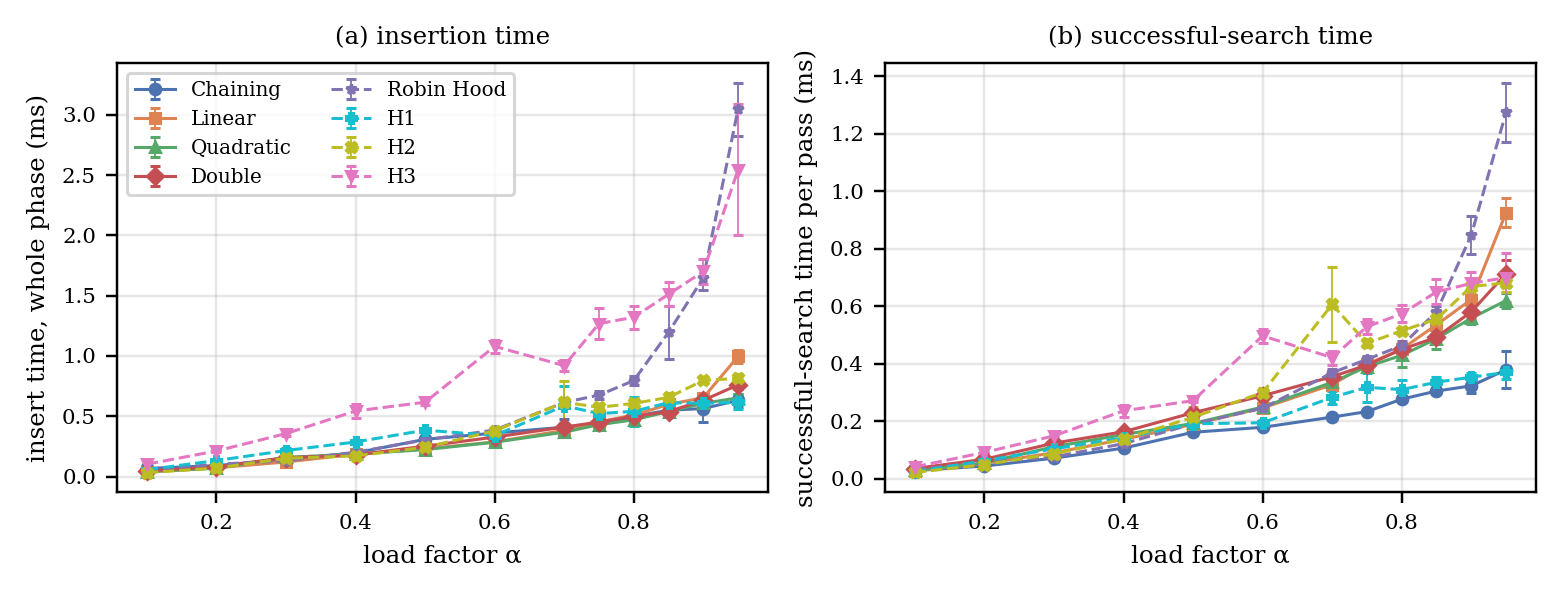
\includegraphics[width=0.92\textwidth]{fig5.png}
\caption{Insertion time (whole insertion phase) and successful-search time per pass versus load factor (mean, bars: 95 \% CI, 30 trials).}
\label{fig:5}
\end{figure*}

Timing curves (Fig. 5, Table 10) are noisy on the virtualized host, which is why we use 30 trials. The jump of double hashing at $\alpha$ = 0.7 that is visible in a single run is not a feature: the 30-trial mean grows monotonically (0.327, 0.410, 0.452 ms at $\alpha$ = 0.6, 0.7, 0.75) with a relative SD of 16 \% at $\alpha$ = 0.7. At $\alpha$ = 0.9 chaining and H1 have the cheapest successful search (0.32 and 0.35 ms per pass) against 0.56--0.68 ms for the open-addressing family, while Robin Hood hashing and H3 pay about 2.5 times the insertion time of linear probing (1.65 and 1.70 ms against 0.65 ms). Chaining insertion is noisy (SD 54 \% at $\alpha$ = 0.9) because of allocator behaviour.

\begin{table}[!t]
\caption{Experiment A times in ms (mean $\pm$ SD, 30 trials; insertion: whole phase; hit: one pass over all keys).}
\label{tab:10}
\centering
\scriptsize
\adjustbox{max width=\columnwidth}{%
\begin{tabular}{|l|l|l|l|l|}
\hline
\textbf{Strategy} & \textbf{Insert $\alpha$=0.5} & \textbf{Hit $\alpha$=0.5} & \textbf{Insert $\alpha$=0.9} & \textbf{Hit $\alpha$=0.9} \\
\hline
Chaining & 0.308 $\pm$ 0.057 & 0.162 $\pm$ 0.023 & 0.564 $\pm$ 0.302 & 0.323 $\pm$ 0.070 \\
Linear & 0.229 $\pm$ 0.021 & 0.189 $\pm$ 0.018 & 0.654 $\pm$ 0.044 & 0.624 $\pm$ 0.046 \\
Quadratic & 0.223 $\pm$ 0.039 & 0.192 $\pm$ 0.015 & 0.607 $\pm$ 0.067 & 0.559 $\pm$ 0.056 \\
Double & 0.252 $\pm$ 0.040 & 0.230 $\pm$ 0.034 & 0.632 $\pm$ 0.082 & 0.581 $\pm$ 0.064 \\
Robin Hood & 0.304 $\pm$ 0.044 & 0.191 $\pm$ 0.024 & 1.648 $\pm$ 0.269 & 0.848 $\pm$ 0.175 \\
H1 & 0.385 $\pm$ 0.046 & 0.191 $\pm$ 0.020 & 0.607 $\pm$ 0.107 & 0.353 $\pm$ 0.036 \\
H2 & 0.242 $\pm$ 0.027 & 0.214 $\pm$ 0.099 & 0.797 $\pm$ 0.050 & 0.668 $\pm$ 0.030 \\
H3 & 0.616 $\pm$ 0.052 & 0.272 $\pm$ 0.011 & 1.700 $\pm$ 0.269 & 0.680 $\pm$ 0.102 \\
\hline
\end{tabular}}
\end{table}


\begin{figure*}[!t]
\centering
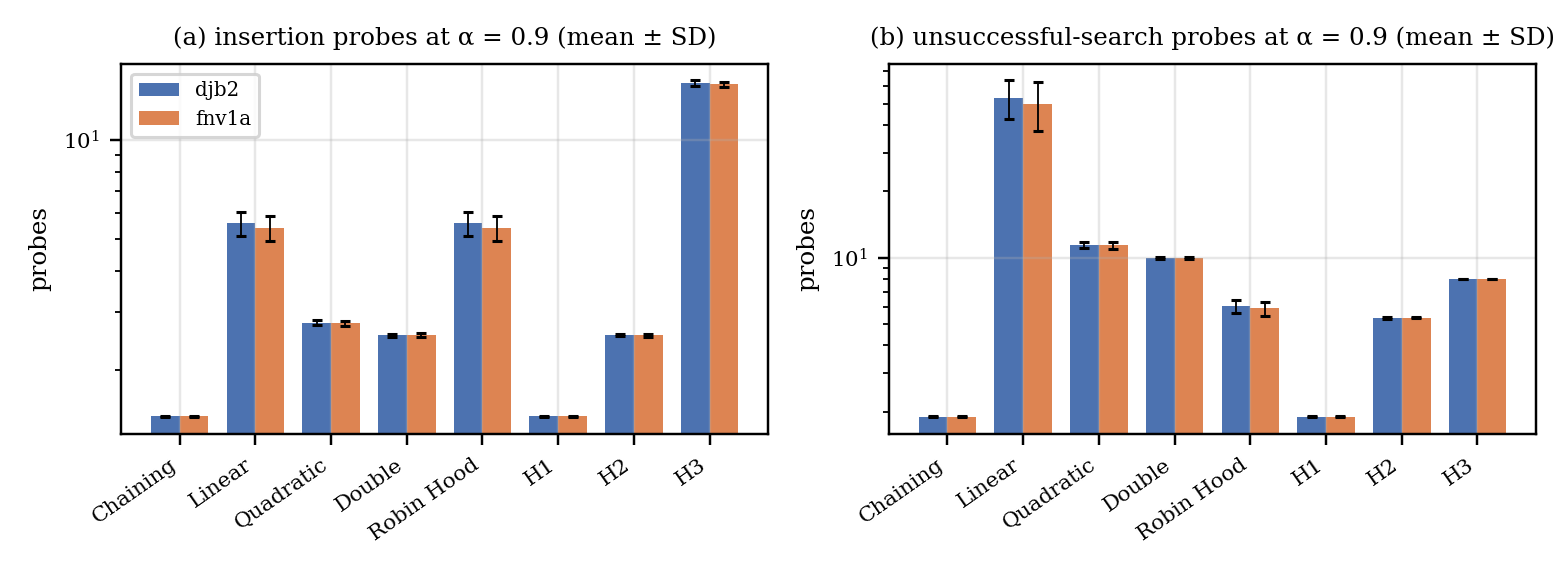
\includegraphics[width=0.92\textwidth]{fig6.png}
\caption{Insertion and unsuccessful-search probes at $\alpha$ = 0.9 for two hash functions (mean $\pm$ SD).}
\label{fig:6}
\end{figure*}

The ranking is the same for the two hash functions (Fig. 6). The insertion failure plot of the earlier version is replaced by one statement: no insertion failed in any of the 5,760 table builds except one H3 insertion at $\alpha$ = 0.95 with FNV-1a, so failures are a capacity and policy outcome that matters only for the stress tests of Section V-D.

\subsection{Probe-Length Distributions}

\begin{figure*}[!t]
\centering
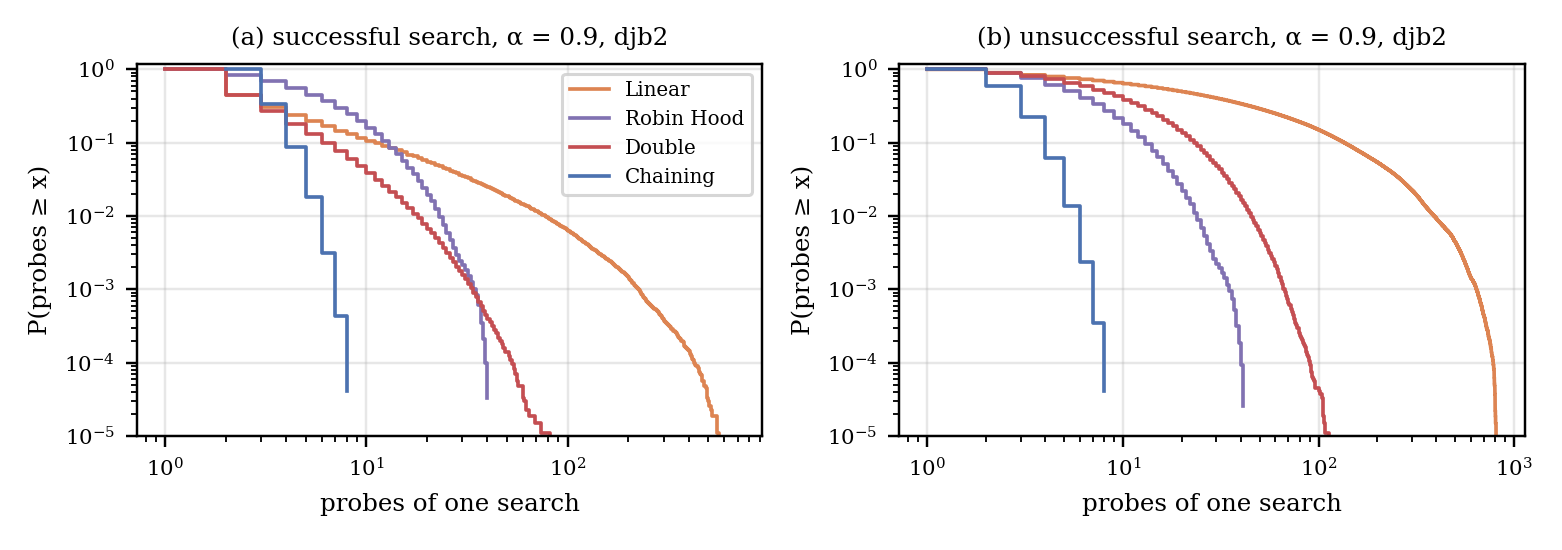
\includegraphics[width=0.92\textwidth]{fig7.png}
\caption{Complementary distribution of the probes of one search at $\alpha$ = 0.9 (djb2, 30 trials pooled).}
\label{fig:7}
\end{figure*}

\begin{table*}[!t]
\caption{Probe-length statistics at $\alpha$ = 0.9 (consistent metric).}
\label{tab:11}
\centering
\scriptsize
\adjustbox{max width=\textwidth}{%
\begin{tabular}{|l|l|l|l|l|l|l|l|l|}
\hline
\textbf{Strategy} & \textbf{Hit mean} & \textbf{Hit var.} & \textbf{Hit p99} & \textbf{Hit max} & \textbf{Miss mean} & \textbf{Miss var.} & \textbf{Miss p99} & \textbf{Miss max} \\
\hline
Linear & 5.49 & 293.2 & 77 & 671 & 49.88 & 6318.9 & 389 & 811 \\
Robin Hood & 5.49 & 22.7 & 22 & 40 & 5.96 & 23.2 & 23 & 41 \\
Double & 2.55 & 10.8 & 17 & 84 & 10.02 & 90.6 & 44 & 113 \\
Chaining & 2.45 & 0.5 & 5 & 8 & 1.90 & 0.9 & 5 & 8 \\
\hline
\end{tabular}}
\end{table*}


Linear probing and Robin Hood hashing share the successful-search mean (5.49) but differ in spread (Table 11, Fig. 7): the variance falls from 293 to 23, the 99th percentile from 77 to 22 and the maximum from 671 to 40 probes. For unsuccessful search Robin Hood hashing also lowers the mean from 49.9 to 6.0 because its early-exit rule stops at the first resident that is closer to home. Chaining has the smallest spread (hit variance 0.5), which matters for latency-sensitive compilation phases.

\subsection{Memory}

\begin{figure}[!t]
\centering
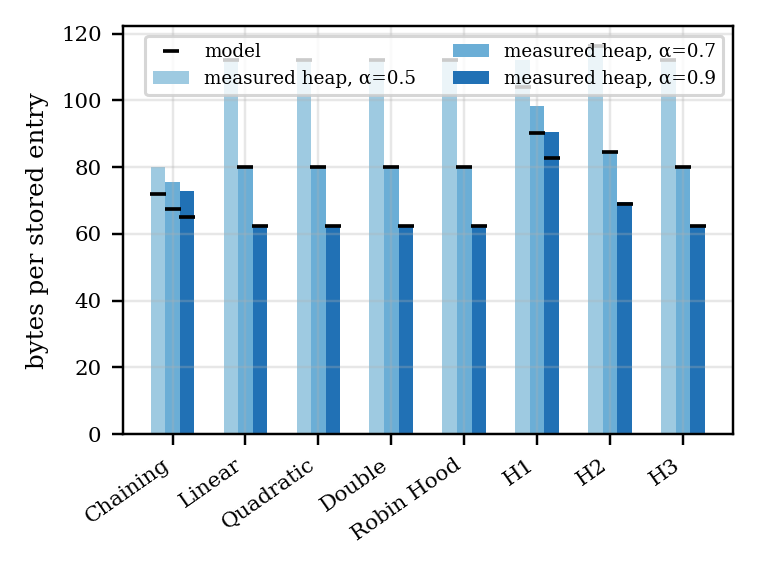
\includegraphics[width=\columnwidth]{fig8.png}
\caption{Table-structure bytes per stored entry: model (ticks) and measured heap (bars) at $\alpha$ = 0.5, 0.7, 0.9.}
\label{fig:8}
\end{figure}

\begin{table*}[!t]
\caption{Bytes per entry: estimation model and measured heap (djb2, mean of 30 trials).}
\label{tab:12}
\centering
\scriptsize
\adjustbox{max width=\textwidth}{%
\begin{tabular}{|l|l|l|l|l|l|l|}
\hline
\textbf{Strategy} & \textbf{$\alpha$=0.5 model} & \textbf{$\alpha$=0.5 heap} & \textbf{$\alpha$=0.7 model} & \textbf{$\alpha$=0.7 heap} & \textbf{$\alpha$=0.9 model} & \textbf{$\alpha$=0.9 heap} \\
\hline
Chaining & 72.0 & 79.9 & 67.4 & 75.4 & 64.9 & 72.8 \\
Linear & 112.0 & 112.0 & 80.0 & 80.0 & 62.2 & 62.2 \\
Quadratic & 112.0 & 112.0 & 80.0 & 80.0 & 62.2 & 62.2 \\
Double & 112.0 & 112.0 & 80.0 & 80.0 & 62.2 & 62.2 \\
Robin Hood & 112.0 & 112.0 & 80.0 & 80.0 & 62.2 & 62.2 \\
H1 & 104.0 & 111.9 & 90.3 & 98.2 & 82.7 & 90.6 \\
H2 & 116.3 & 116.3 & 84.5 & 84.6 & 69.1 & 69.7 \\
H3 & 112.1 & 112.1 & 80.1 & 80.1 & 62.3 & 62.3 \\
\hline
\end{tabular}}
\end{table*}


The estimate counts only table structure: bytes = (slots $\times$ slot size + allocated nodes $\times$ node size) / stored entries, with sizeof(Symbol) = 48 B on this platform, a list node 56 B, an open-addressing slot 56 B, an H1 bucket header 24 B and a tree entry 112 B. Identifiers of at most 15 characters fit the string's inline buffer, so key bytes are inside the symbol. The earlier text and figure disagreed because the figure plotted $\alpha$ = 0.7 (chaining 67.4, open addressing 80.0, H1 90.3, H2 84.5 B) while the text quoted $\alpha$ = 0.9 (64.9, 62.2, 82.7, 69.1 B); both are correct for their load factor (Table 12). Chaining looks cheapest at low and medium load because it allocates only the nodes it stores (8/$\alpha$ + 56 B per entry), whereas open addressing pre-allocates every slot (56/$\alpha$ B); the model crosses at $\alpha$ $\approx$ 0.86. The model ignores allocator overhead: measured heap bytes (glibc mallinfo2) are 7.9 B per entry higher for chaining (one 8-byte malloc header per node) and 7.9 B higher for H1, so the measured crossover is near $\alpha$ $\approx$ 0.75. For slot arrays the measurement equals the model to within 0.1 B.

\subsection{Do the Hybrids Use Their Special Mechanisms?}

\begin{table*}[!t]
\caption{Hybrid-mechanism counters in Experiment A (mean per trial, djb2).}
\label{tab:13}
\centering
\scriptsize
\adjustbox{max width=\textwidth}{%
\begin{tabular}{|l|l|l|l|l|l|l|l|}
\hline
\textbf{Strategy} & \textbf{$\alpha$} & \textbf{Keys} & \textbf{Tree conv.} & \textbf{Overflow spills} & \textbf{Overflow walks} & \textbf{Stash} & \textbf{Collisions / kicks} \\
\hline
H1 & 0.50 & 5,003 & 0.0 & -- & -- & -- & 1060 \\
H1 & 0.90 & 9,006 & 0.0 & -- & -- & -- & 3062 \\
H1 & 0.95 & 9,506 & 0.0 & -- & -- & -- & 3367 \\
H2 & 0.50 & 5,003 & -- & 25.9 & 970.0 & -- & 1246 \\
H2 & 0.90 & 9,006 & -- & 741.2 & 21786.5 & -- & 3944 \\
H2 & 0.95 & 9,506 & -- & 968.9 & 26909.2 & -- & 4359 \\
H3 & 0.50 & 5,003 & -- & -- & -- & 0.0 & 22 \\
H3 & 0.90 & 9,006 & -- & -- & -- & 0.0 & 3659 \\
H3 & 0.95 & 9,506 & -- & -- & -- & 0.5 & 10466 \\
\hline
\end{tabular}}
\end{table*}


In Experiment A, H1 behaves exactly like chaining: in 719 of its 720 builds (30 trials $\times$ 12 loads $\times$ 2 hashes) no chain exceeded 8 entries, and a single tree conversion occurred in total (Table 13). H1's curves therefore coincide with those of chaining. H2 does use its overflow chain: at $\alpha$ = 0.9 an average of 741 of 9,006 keys (8.2 \%) spill, and the chain is walked about 21,800 times per trial; H3 placed 28 keys in its stash over all builds, with a mean of 0.5 per trial at $\alpha$ = 0.95. To exercise the mechanisms we added stress scenarios (Table 14): random keys with the weak sum hash, and 256 and 4,096 keys that share one djb2 value (concatenations of the blocks ``ab'' and ``bA'', which have equal djb2 contribution), the hash-flooding case [20].

\begin{table*}[!t]
\caption{Stress tests at fixed capacity 10,007 (probes on the consistent metric; mechanism counts for H1: tree conversions, H2: spills / overflow walks, H3: stashed keys / kicks).}
\label{tab:14}
\centering
\scriptsize
\adjustbox{max width=\textwidth}{%
\begin{tabular}{|l|l|l|l|l|l|l|l|}
\hline
\textbf{Scenario} & \textbf{Strategy} & \textbf{Keys} & \textbf{Insert probes} & \textbf{Hit probes} & \textbf{Miss probes} & \textbf{Failed} & \textbf{Mechanism count} \\
\hline
random-djb2-$\alpha$0.9 & Chaining & 9,006 & 1.5 & 2.5 & 1.9 & 0 & -- \\
random-djb2-$\alpha$0.9 & H1 & 9,006 & 1.5 & 2.5 & 1.9 & 0 & 0 conversions \\
random-djb2-$\alpha$0.9 & Linear & 9,006 & 5.3 & 5.3 & 49.2 & 0 & -- \\
random-djb2-$\alpha$0.9 & H2 & 9,006 & 2.6 & 2.6 & 5.3 & 0 & 792 spills / 2386 chain walks \\
random-djb2-$\alpha$0.9 & H3 & 9,006 & 14.6 & 3.6 & 8.0 & 0 & 0 stashed / 3387 kicks \\
random-sum-$\alpha$0.9 & Chaining & 9,006 & 4.7 & 5.7 & 8.5 & 0 & -- \\
random-sum-$\alpha$0.9 & H1 & 9,006 & 4.3 & 4.8 & 6.1 & 0 & 414 conversions \\
random-sum-$\alpha$0.9 & Linear & 9,006 & 3892.6 & 3892.6 & 8382.0 & 0 & -- \\
random-sum-$\alpha$0.9 & H2 & 9,006 & 10.8 & 10.8 & 14.5 & 0 & 7702 spills / 11678 chain walks \\
random-sum-$\alpha$0.9 & H3 & 9,006 & 102.1 & 5.3 & 12.0 & 295 & 4 stashed / 89605 kicks \\
collide-djb2-256 & Chaining & 256 & 128.5 & 129.5 & 2.0 & 0 & -- \\
collide-djb2-256 & H1 & 256 & 8.1 & 10.0 & 1.0 & 0 & 1 conversions \\
collide-djb2-256 & Linear & 256 & 128.5 & 128.5 & 3.5 & 0 & -- \\
collide-djb2-256 & H2 & 256 & 128.5 & 128.5 & 1.0 & 0 & 248 spills / 249 chain walks \\
collide-djb2-256 & H3 & 256 & 13.0 & 5.0 & 8.0 & 0 & 0 stashed / 0 kicks \\
collide-djb2-4096 & Chaining & 4,096 & 2048.5 & 2049.5 & 2.0 & 0 & -- \\
collide-djb2-4096 & H1 & 4,096 & 12.0 & 14.0 & 1.0 & 0 & 1 conversions \\
collide-djb2-4096 & Linear & 4,096 & 2048.5 & 2048.5 & 863.7 & 0 & -- \\
collide-djb2-4096 & H2 & 4,096 & 2048.5 & 2048.5 & 1.0 & 0 & 4088 spills / 4089 chain walks \\
collide-djb2-4096 & H3 & 4,096 & 58.7 & 5.9 & 12.0 & 94 & 4 stashed / 19609 kicks \\
\hline
\end{tabular}}
\end{table*}


With the weak sum hash at $\alpha$ = 0.9, H1 converted 414 chains to trees and lowered the miss cost from 8.5 (chaining) to 6.1 probes; H2 spilled 7,702 of 9,006 keys to its overflow chain, and H3 failed to place 295 keys because both candidate buckets and the stash were full. With 4,096 keys of one djb2 value, chaining needs 2050 probes per successful search, H1 only 14; H2's window does not help hits (2,049) but keeps misses at 1.0 because a miss stops at the first empty slot; H3 spreads colliding keys through its second hash but still rejected 94 keys at fixed capacity. The mechanisms thus work as designed, and each trades a cost: tree nodes (memory), overflow chains (pointer walks) and rebuilds or failures (cuckoo).

\subsection{Scope-Handling Designs}

\begin{figure*}[!t]
\centering
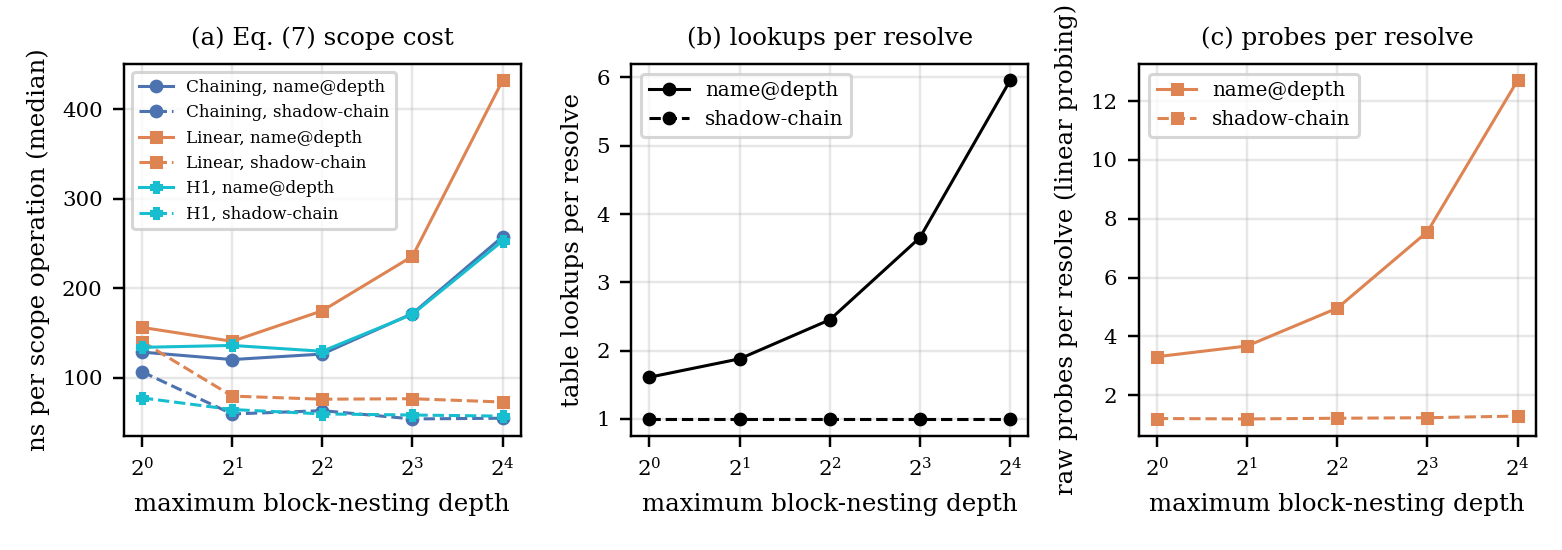
\includegraphics[width=0.92\textwidth]{fig9.png}
\caption{Scope cost of the two designs versus maximum nesting depth (median of 7 repetitions): (a) Eq. (7) in ns per scope operation, (b) table lookups per resolve, (c) raw probes per resolve under linear probing.}
\label{fig:9}
\end{figure*}

\begin{table*}[!t]
\caption{Scope cost, Eq. (7), median (interquartile range) over 7 repetitions, djb2, resizing tables; 80 \% of resolves target a visible name.}
\label{tab:15}
\centering
\scriptsize
\adjustbox{max width=\textwidth}{%
\begin{tabular}{|l|l|l|l|l|l|l|}
\hline
\textbf{Depth} & \textbf{Strategy} & \textbf{name@depth, ns/op} & \textbf{Shadow chain, ns/op} & \textbf{Ratio} & \textbf{Lookups / resolve name@d} & \textbf{Lookups / resolve shadow} \\
\hline
2 & Chaining & 120 (119--123) & 60 (59--61) & 2.02$\times$ & 1.88 & 1.00 \\
2 & Linear & 141 (140--147) & 80 (79--80) & 1.77$\times$ & 1.88 & 1.00 \\
2 & Quadratic & 141 (140--142) & 87 (83--89) & 1.63$\times$ & 1.88 & 1.00 \\
2 & Double & 164 (156--167) & 99 (97--101) & 1.65$\times$ & 1.88 & 1.00 \\
2 & Robin Hood & 122 (112--150) & 58 (57--59) & 2.09$\times$ & 1.88 & 1.00 \\
2 & H1 & 136 (125--157) & 65 (65--72) & 2.10$\times$ & 1.88 & 1.00 \\
2 & H2 & 144 (141--151) & 76 (76--79) & 1.89$\times$ & 1.88 & 1.00 \\
2 & H3 & 167 (164--175) & 119 (115--121) & 1.40$\times$ & 1.88 & 1.00 \\
8 & Chaining & 172 (166--177) & 54 (53--55) & 3.17$\times$ & 3.65 & 1.00 \\
8 & Linear & 236 (230--240) & 77 (76--78) & 3.07$\times$ & 3.65 & 1.00 \\
8 & Quadratic & 238 (233--269) & 87 (84--91) & 2.73$\times$ & 3.65 & 1.00 \\
8 & Double & 237 (233--252) & 84 (82--85) & 2.82$\times$ & 3.65 & 1.00 \\
8 & Robin Hood & 157 (150--161) & 54 (53--54) & 2.93$\times$ & 3.65 & 1.00 \\
8 & H1 & 171 (170--176) & 59 (58--60) & 2.92$\times$ & 3.65 & 1.00 \\
8 & H2 & 204 (198--212) & 73 (72--76) & 2.81$\times$ & 3.65 & 1.00 \\
8 & H3 & 258 (250--261) & 98 (96--98) & 2.63$\times$ & 3.65 & 1.00 \\
\hline
\end{tabular}}
\end{table*}


We replayed identical block-structured programs (150 top-level blocks, each nesting down to the maximum depth, 3--10 declarations and 10--29 resolves per block, 600 names) on both designs and on every strategy; both designs agreed with a reference model on every resolve. At depth 8 the name@depth design needs 3.65 table lookups per resolve (each with a string concatenation) against 1.00 for the shadow chain, and is 2.6--3.2 times slower per scope operation, depending on the strategy (Table 15, Fig. 9a). At depth 2 the factor is 1.4--2.1. The cost of name@depth grows with nesting depth (Fig. 9b), whereas the shadow chain is nearly independent of it; its price is one lookup in each declaration and the restore work at scope exit. The shadow chain also helps open addressing disproportionately, because unsuccessful lookups of name@d keys for each outer depth are the expensive case there: under linear probing the raw probes per resolve fall from 7.6 to 1.2 at depth 8 (Fig. 9c). Name@depth remains attractive for its simplicity, but a compiler with deep nesting should prefer shadow chains.

\subsection{Experiment B: Resizing, Deletion and Workloads}

\textbf{Audit.} The earlier summary of this experiment mentioned ``very large'' values and asked for an audit. We re-examined every column of the benchmark. Units are correct: times are nanoseconds per operation (total milliseconds $\times$ 10\textsuperscript{6} $\div$ operations), and the implied time per probe lies between 9 and 60 ns (5th--95th percentile; median 31 ns) in all 1,288 runs, which is plausible for cache-missing string comparisons and rules out a factor error. The large values come from the weak sum hash: pooled over the three synthetic workloads, the mean number of probes of a successful search is 1,153 for sum against 1.65--4.82 for the four other hashes, so any average that pools hash functions is dominated by the weak one. Three genuine defects were fixed: (i) results were pooled across hash functions and workloads, so we now report each workload $\times$ hash $\times$ strategy cell; (ii) each cell was a single run, so we now report the median of 5 repetitions; (iii) the column max\_probe mixed insertion and lookup maxima, which we now keep apart in the CSV. All 1,288 runs passed the correctness checks (stored keys found, absent keys absent, deleted keys gone).

\begin{table*}[!t]
\caption{Experiment B, djb2: median insertion time in ns per key, including resizing (n: unique keys of the workload).}
\label{tab:16}
\centering
\scriptsize
\adjustbox{max width=\textwidth}{%
\begin{tabular}{|l|l|l|l|l|l|l|l|}
\hline
\textbf{Strategy} & \textbf{random} & \textbf{seq.} & \textbf{code} & \textbf{lua ids} & \textbf{zlib ids} & \textbf{redis ids} & \textbf{sqlite ids} \\
\textbf{n keys} & \textbf{30,000} & \textbf{30,000} & \textbf{30,000} & \textbf{3,351} & \textbf{878} & \textbf{12,833} & \textbf{13,835} \\
\hline
Chaining & 107 & 58 & 138 & 101 & 121 & 145 & 215 \\
Linear & 148 & 148 & 304 & 148 & 113 & 235 & 216 \\
Quadratic & 168 & 91 & 271 & 150 & 114 & 255 & 200 \\
Double & 176 & 126 & 272 & 139 & 121 & 323 & 205 \\
Robin Hood & 183 & 276 & 255 & 189 & 112 & 269 & 202 \\
H1 & 270 & 169 & 385 & 253 & 154 & 434 & 355 \\
H2 & 205 & 163 & 284 & 155 & 98 & 274 & 253 \\
H3 & 312 & 264 & 421 & 324 & 199 & 466 & 410 \\
\hline
\end{tabular}}
\end{table*}


\begin{table*}[!t]
\caption{Experiment B, djb2: median successful-search time in ns.}
\label{tab:17}
\centering
\scriptsize
\adjustbox{max width=\textwidth}{%
\begin{tabular}{|l|l|l|l|l|l|l|l|}
\hline
\textbf{Strategy} & \textbf{random} & \textbf{seq.} & \textbf{code} & \textbf{lua ids} & \textbf{zlib ids} & \textbf{redis ids} & \textbf{sqlite ids} \\
\textbf{n keys} & \textbf{30,000} & \textbf{30,000} & \textbf{30,000} & \textbf{3,351} & \textbf{878} & \textbf{12,833} & \textbf{13,835} \\
\hline
Chaining & 49 & 41 & 69 & 28 & 30 & 50 & 90 \\
Linear & 51 & 59 & 71 & 39 & 39 & 53 & 54 \\
Quadratic & 49 & 52 & 70 & 39 & 41 & 71 & 51 \\
Double & 74 & 57 & 82 & 40 & 47 & 97 & 57 \\
Robin Hood & 45 & 78 & 65 & 33 & 24 & 51 & 42 \\
H1 & 52 & 46 & 75 & 38 & 24 & 58 & 55 \\
H2 & 50 & 55 & 69 & 35 & 27 & 60 & 51 \\
H3 & 77 & 64 & 99 & 60 & 51 & 88 & 80 \\
\hline
\end{tabular}}
\end{table*}


\begin{table*}[!t]
\caption{Experiment B, djb2: median unsuccessful-search time in ns.}
\label{tab:18}
\centering
\scriptsize
\adjustbox{max width=\textwidth}{%
\begin{tabular}{|l|l|l|l|l|l|l|l|}
\hline
\textbf{Strategy} & \textbf{random} & \textbf{seq.} & \textbf{code} & \textbf{lua ids} & \textbf{zlib ids} & \textbf{redis ids} & \textbf{sqlite ids} \\
\textbf{n keys} & \textbf{30,000} & \textbf{30,000} & \textbf{30,000} & \textbf{3,351} & \textbf{878} & \textbf{12,833} & \textbf{13,835} \\
\hline
Chaining & 30 & 30 & 38 & 23 & 28 & 32 & 47 \\
Linear & 59 & 77 & 68 & 44 & 50 & 54 & 58 \\
Quadratic & 59 & 76 & 68 & 46 & 51 & 66 & 52 \\
Double & 71 & 70 & 73 & 44 & 51 & 86 & 63 \\
Robin Hood & 45 & 55 & 49 & 30 & 25 & 50 & 41 \\
H1 & 35 & 39 & 43 & 25 & 21 & 38 & 36 \\
H2 & 59 & 60 & 66 & 39 & 34 & 60 & 56 \\
H3 & 100 & 91 & 100 & 84 & 68 & 96 & 96 \\
\hline
\end{tabular}}
\end{table*}


\begin{table*}[!t]
\caption{Experiment B, djb2: median deletion time in ns (every second key deleted).}
\label{tab:19}
\centering
\scriptsize
\adjustbox{max width=\textwidth}{%
\begin{tabular}{|l|l|l|l|l|l|l|l|}
\hline
\textbf{Strategy} & \textbf{random} & \textbf{seq.} & \textbf{code} & \textbf{lua ids} & \textbf{zlib ids} & \textbf{redis ids} & \textbf{sqlite ids} \\
\textbf{n keys} & \textbf{30,000} & \textbf{30,000} & \textbf{30,000} & \textbf{3,351} & \textbf{878} & \textbf{12,833} & \textbf{13,835} \\
\hline
Chaining & 64 & 55 & 95 & 40 & 54 & 81 & 133 \\
Linear & 56 & 72 & 73 & 38 & 44 & 62 & 61 \\
Quadratic & 54 & 61 & 72 & 39 & 46 & 73 & 58 \\
Double & 81 & 58 & 82 & 40 & 52 & 102 & 69 \\
Robin Hood & 69 & 109 & 87 & 49 & 47 & 78 & 68 \\
H1 & 66 & 64 & 100 & 44 & 43 & 96 & 83 \\
H2 & 50 & 62 & 70 & 36 & 35 & 65 & 65 \\
H3 & 90 & 69 & 106 & 75 & 59 & 96 & 95 \\
\hline
\end{tabular}}
\end{table*}


\begin{table*}[!t]
\caption{Experiment B, djb2: Eq. (7) scope cost in ns per scope operation (name@depth design).}
\label{tab:20}
\centering
\scriptsize
\adjustbox{max width=\textwidth}{%
\begin{tabular}{|l|l|l|l|l|l|l|l|}
\hline
\textbf{Strategy} & \textbf{random} & \textbf{seq.} & \textbf{code} & \textbf{lua ids} & \textbf{zlib ids} & \textbf{redis ids} & \textbf{sqlite ids} \\
\textbf{n keys} & \textbf{30,000} & \textbf{30,000} & \textbf{30,000} & \textbf{3,351} & \textbf{878} & \textbf{12,833} & \textbf{13,835} \\
\hline
Chaining & 114 & 96 & 191 & 97 & 119 & 149 & 210 \\
Linear & 165 & 135 & 219 & 156 & 165 & 220 & 212 \\
Quadratic & 185 & 150 & 218 & 148 & 174 & 237 & 212 \\
Double & 204 & 154 & 213 & 155 & 176 & 332 & 215 \\
Robin Hood & 146 & 117 & 166 & 110 & 94 & 197 & 176 \\
H1 & 116 & 100 & 163 & 107 & 87 & 172 & 158 \\
H2 & 170 & 144 & 206 & 159 & 133 & 226 & 222 \\
H3 & 228 & 196 & 252 & 222 & 164 & 254 & 269 \\
\hline
\end{tabular}}
\end{table*}


With djb2 and well-distributed identifiers (Table 16--Table 20) most strategies are within noise of each other in time for successful search (roughly 25--100 ns); the clear separations are those that probe counts predict. Chaining and H1 have the cheapest unsuccessful searches (23--47 and 21--43 ns) and H3 the most expensive (68--100 ns, always two buckets). Robin Hood hashing is the fastest, or within 5 ns of the fastest, for successful search on all four real-code sets. Insertion including resizing is cheapest for chaining on synthetic keys (58--138 ns) and costs 2.5--4.5 times more for H1 and H3, which pay for tree bookkeeping and displacement. H1 never converted a chain to a tree with djb2 on any of the seven workloads, so on real identifiers it behaves exactly as chaining; the weak-hash block below is where it differs. Real identifier sets (lua, zlib, redis, sqlite) behave like the random workload; the sequential workload is harder for linear probing and Robin Hood hashing under djb2 (successful-search probes 3.96 against 1.42 on random keys) while double hashing is unaffected (1.37).

\begin{table*}[!t]
\caption{Experiment B: unsuccessful-search probes (consistent metric, median) for each hash function on three workloads (random and sequential: 30,000 keys, 10,000 for the sum hash; SQLite: 13,835 keys, 10,000 for sum).}
\label{tab:21}
\centering
\scriptsize
\adjustbox{max width=\textwidth}{%
\begin{tabular}{|l|l|l|l|l|l|l|l|l|l|l|l|l|l|l|l|}
\hline
 & \textbf{random} &  &  &  &  & \textbf{sequential} &  &  &  &  & \textbf{sqlite ids} &  &  &  &  \\
\textbf{Strategy} & \textbf{djb2} & \textbf{fnv1a} & \textbf{sdbm} & \textbf{pjw} & \textbf{sum} & \textbf{djb2} & \textbf{fnv1a} & \textbf{sdbm} & \textbf{pjw} & \textbf{sum} & \textbf{djb2} & \textbf{fnv1a} & \textbf{sdbm} & \textbf{pjw} & \textbf{sum} \\
\hline
Chaining & 1.45 & 1.45 & 1.46 & 1.45 & 9.24 & 1.51 & 1.45 & 1.45 & 1.61 & 44.02 & 1.42 & 1.43 & 1.42 & 1.42 & 5.67 \\
Linear & 2.22 & 2.17 & 2.19 & 2.34 & 9359.27 & 6.82 & 2.07 & 5.94 & 196.76 & 9773.84 & 2.11 & 1.99 & 2.04 & 2.90 & 8841.75 \\
Quadratic & 1.96 & 1.93 & 1.94 & 2.02 & 97.67 & 3.25 & 1.92 & 2.61 & 8.95 & 87.18 & 1.85 & 1.82 & 1.82 & 1.88 & 94.86 \\
Double & 1.82 & 1.82 & 1.83 & 1.83 & 4.74 & 1.88 & 1.83 & 1.83 & 2.00 & 3.63 & 1.72 & 1.73 & 1.72 & 1.71 & 4.93 \\
Robin Hood & 1.65 & 1.63 & 1.65 & 1.67 & 4567.66 & 2.89 & 1.61 & 2.25 & 21.64 & 7235.74 & 1.59 & 1.58 & 1.58 & 1.68 & 3940.17 \\
H1 & 1.45 & 1.45 & 1.46 & 1.45 & 5.95 & 1.51 & 1.45 & 1.45 & 1.61 & 2.68 & 1.42 & 1.43 & 1.42 & 1.42 & 4.91 \\
H2 & 2.11 & 2.09 & 2.10 & 2.15 & 15.20 & 3.51 & 2.04 & 3.33 & 4.10 & 45.88 & 1.98 & 1.93 & 1.95 & 2.01 & 11.43 \\
H3 & 8.00 & 8.00 & 8.00 & 8.00 & 8.00 & 8.00 & 8.00 & 8.00 & 8.00 & 10.00 & 8.00 & 8.00 & 8.00 & 8.00 & 8.00 \\
\hline
\end{tabular}}
\end{table*}


\begin{figure*}[!t]
\centering
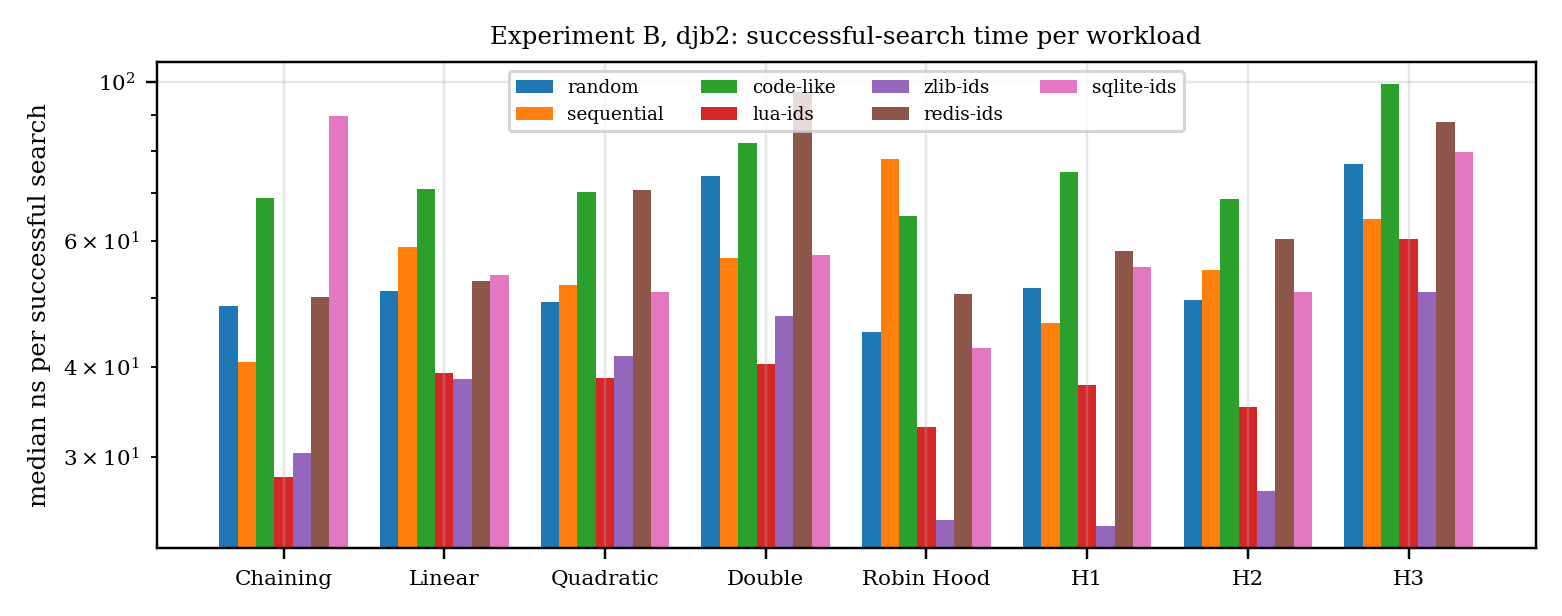
\includegraphics[width=0.92\textwidth]{fig10.png}
\caption{Experiment B, djb2: successful-search time per workload (median ns, log scale).}
\label{fig:10}
\end{figure*}

\begin{figure*}[!t]
\centering
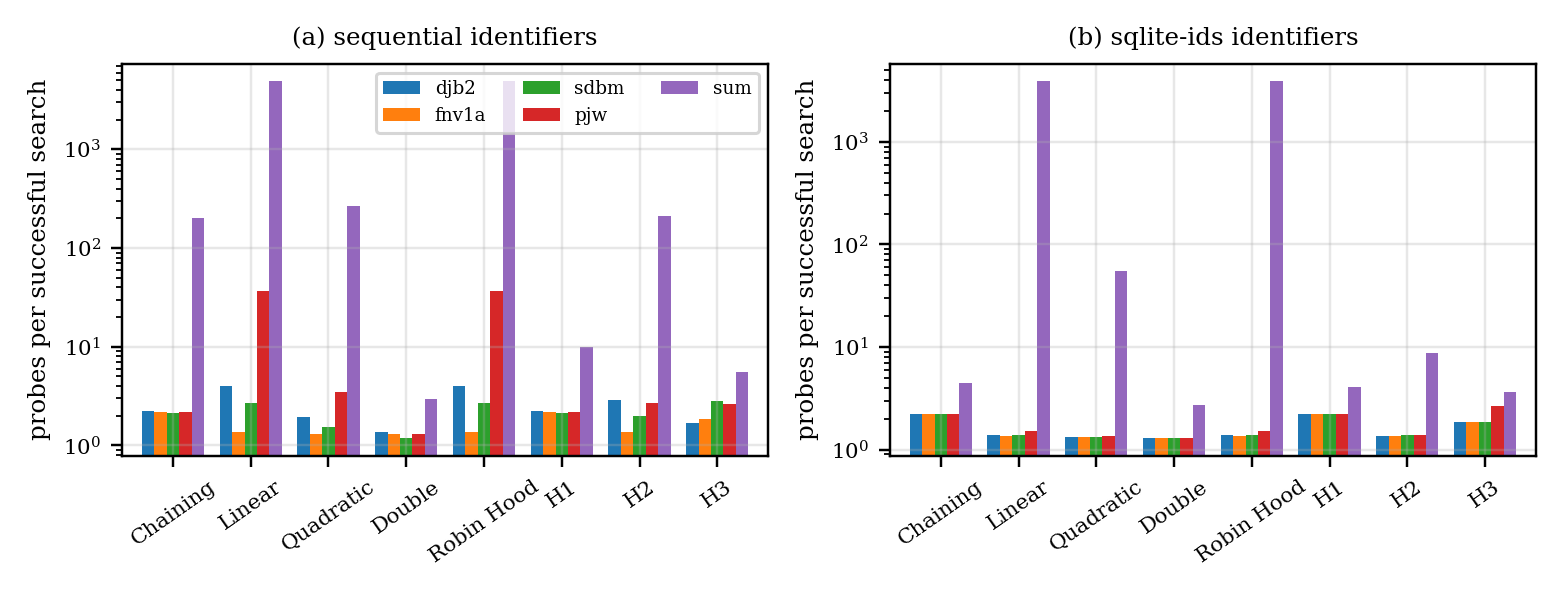
\includegraphics[width=0.92\textwidth]{fig11.png}
\caption{Hash-function sensitivity: successful-search probes (consistent metric, median) on sequential identifiers and on the SQLite identifier set.}
\label{fig:11}
\end{figure*}

Hash functions (Table 21, Fig. 11) matter little for the four regular hashes on random and real identifiers, but the weak sum hash is catastrophic for open addressing: on sequential identifiers the miss cost is 9,774 probes for linear probing and 7,236 for Robin Hood hashing, against 44 for chaining, 46 for H2, 3.6 for double hashing and 2.7 for H1, whose trees bound the damage. On the SQLite identifiers the same pattern holds (8,842 and 3,940 against 5.7 for chaining and 4.9 for H1). PJW was the weakest of the regular hashes on sequential names (linear-probing miss cost 197 against 2.1 for FNV-1a), so a hash function must be tested on realistic identifier patterns and not only on random strings.

\begin{table*}[!t]
\caption{Hybrid mechanisms under the weak sum hash in Experiment B (median of 3 runs).}
\label{tab:22}
\centering
\scriptsize
\adjustbox{max width=\textwidth}{%
\begin{tabular}{|l|l|l|l|l|l|l|l|}
\hline
\textbf{Workload} & \textbf{Strategy} & \textbf{Keys} & \textbf{Hit probes} & \textbf{Miss probes} & \textbf{Tree conv.} & \textbf{Overflow spills} & \textbf{Stashed} \\
\hline
random & H1 & 10,000 & 4.9 & 5.9 & 637 & 0 & 0 \\
random & H2 & 10,000 & 11.4 & 15.2 & 0 & 8,699 & 0 \\
random & H3 & 10,000 & 4.7 & 8.0 & 0 & 0 & 0 \\
sequential & H1 & 10,000 & 9.9 & 2.7 & 211 & 0 & 0 \\
sequential & H2 & 10,000 & 209.6 & 45.9 & 0 & 9,888 & 0 \\
sequential & H3 & 10,000 & 5.5 & 10.0 & 0 & 0 & 22 \\
code-like & H1 & 10,000 & 4.7 & 5.3 & 501 & 0 & 0 \\
code-like & H2 & 10,000 & 10.8 & 13.2 & 0 & 8,268 & 0 \\
code-like & H3 & 10,000 & 4.4 & 8.0 & 0 & 0 & 0 \\
\hline
\end{tabular}}
\end{table*}


Under the sum hash (Table 22) all three mechanisms are active: H1 converts hundreds of chains (637 on random, 211 on sequential and 501 on code-like keys), H2 spills 83--99 \% of its keys, and H3 stashed keys on sequential identifiers.

\subsection{Real Compiler Workloads}

\begin{table*}[!t]
\caption{Flat replay of identifier tokens, djb2: median ns per access and consistent probes per access (including insertions on first occurrence).}
\label{tab:23}
\centering
\scriptsize
\adjustbox{max width=\textwidth}{%
\begin{tabular}{|l|l|l|l|l|l|l|l|l|}
\hline
\textbf{Strategy} & \textbf{Lua ns} & \textbf{Lua pr.} & \textbf{zlib ns} & \textbf{zlib pr.} & \textbf{Redis ns} & \textbf{Redis pr.} & \textbf{SQLite ns} & \textbf{SQLite pr.} \\
\hline
Chaining & 36 & 2.31 & 28 & 2.25 & 39 & 2.28 & 35 & 2.30 \\
Linear & 51 & 2.33 & 36 & 1.80 & 51 & 2.18 & 65 & 2.12 \\
Quadratic & 48 & 1.87 & 37 & 1.61 & 49 & 1.84 & 52 & 1.78 \\
Double & 46 & 1.72 & 35 & 1.48 & 58 & 1.73 & 55 & 1.69 \\
Robin Hood & 49 & 2.16 & 33 & 1.74 & 48 & 1.96 & 52 & 1.96 \\
H1 & 45 & 2.31 & 29 & 2.25 & 50 & 2.28 & 51 & 2.30 \\
H2 & 44 & 1.96 & 31 & 1.69 & 50 & 1.95 & 48 & 1.89 \\
H3 & 67 & 4.61 & 54 & 3.69 & 86 & 4.23 & 78 & 4.09 \\
\hline
\end{tabular}}
\end{table*}


\begin{figure*}[!t]
\centering
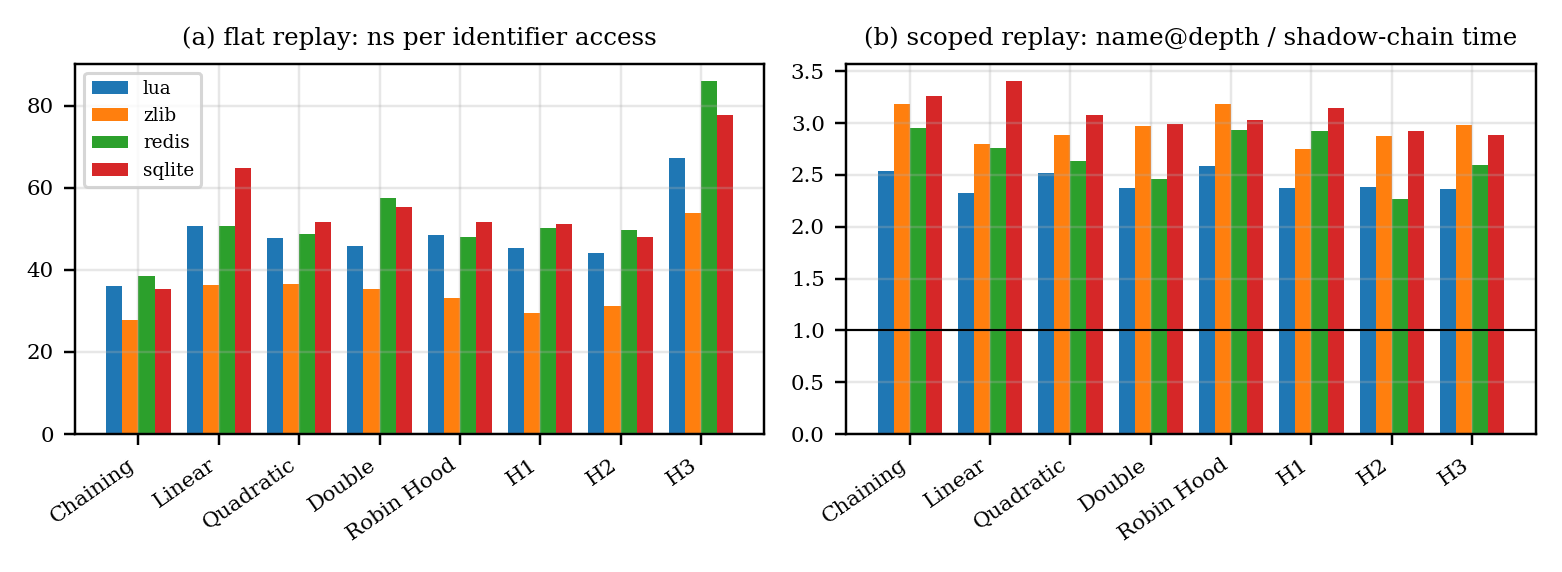
\includegraphics[width=0.92\textwidth]{fig12.png}
\caption{Real-code replays (djb2): (a) flat replay, ns per identifier access; (b) scoped replay, time of name@depth relative to the shadow chain.}
\label{fig:12}
\end{figure*}

The four corpora contain 547,703 identifier tokens; 84--89 \% of the accesses of a flat replay are hits, as in a real compiler, where most tokens repeat an identifier already seen (Table 23, Fig. 12a). Chaining and H1 are fastest (28--51 ns per access, 2.25--2.31 probes), double hashing needs the fewest probes (1.48--1.73), H3 the most (3.7--4.6) and is the slowest (54--86 ns). Chaining and H1 are identical in probes on all four corpora because no chain exceeded eight entries.

\begin{table*}[!t]
\caption{Block-scoped replay of real code, djb2: median ns per scope operation for both designs, and table lookups per resolve in the last row (the shadow-chain count includes the lookup made by each declaration).}
\label{tab:24}
\centering
\scriptsize
\adjustbox{max width=\textwidth}{%
\begin{tabular}{|l|l|l|l|l|l|l|l|l|}
\hline
\textbf{Strategy} & \textbf{Lua name@d} & \textbf{Lua shadow} & \textbf{zlib name@d} & \textbf{zlib shadow} & \textbf{Redis name@d} & \textbf{Redis shadow} & \textbf{SQLite name@d} & \textbf{SQLite shadow} \\
\hline
Chaining & 96 & 38 & 92 & 29 & 120 & 41 & 119 & 36 \\
Linear & 126 & 54 & 107 & 38 & 146 & 53 & 188 & 55 \\
Quadratic & 129 & 51 & 102 & 35 & 140 & 53 & 182 & 59 \\
Double & 116 & 49 & 108 & 36 & 148 & 60 & 168 & 56 \\
Robin Hood & 96 & 37 & 90 & 28 & 128 & 43 & 135 & 45 \\
H1 & 91 & 38 & 86 & 31 & 113 & 39 & 131 & 42 \\
H2 & 109 & 46 & 98 & 34 & 143 & 63 & 153 & 53 \\
H3 & 148 & 63 & 153 & 51 & 190 & 73 & 209 & 72 \\
lookups / resolve & 2.14 & 1.17 & 2.44 & 1.09 & 2.35 & 1.13 & 2.61 & 1.12 \\
\hline
\end{tabular}}
\end{table*}


In the scoped replay (Table 24, Fig. 12b) the shadow chain is 2.3--3.4 times faster than name@depth on every corpus and strategy, because real code resolves against a depth of up to 10 with 48--57 \% of uses resolving to a heuristically detected declaration, so unsuccessful resolves, such as globals and library names not declared in the file, walk the whole chain of depths (2.1--2.6 lookups per resolve against 1.1--1.2). The declaration heuristic misses declarations that do not follow a type name, which understates the hit ratio and favours the shadow chain slightly; we therefore report the direction of the effect, not its precise size.

\section{Verification}

The C++ test suite runs 1,440,178 checks (hash test vectors, edge cases, scope behaviour, and differential fuzzing against std::unordered\_map [29]) under AddressSanitizer and UndefinedBehaviorSanitizer [30], [31]; it passes after the counters and the shadow-chain scope manager were added. Every benchmark run verifies that stored keys are found, absent keys are not returned and deleted keys are gone (1,288 Experiment B runs, 5,760 Experiment A builds, and the trace replays all passed). Both scope designs agree with an independent reference model on every resolve of the scope experiment. A JavaScript engine reproduces the C++ engine on identical operation scripts (26,640 counters compared) and passes 433,531 engine checks; browser timings include JIT effects and are for demonstration only. Four issues were corrected before the evaluation: a link error without -O2 (odr-use of static constants), a missing digit in the FNV-1a offset basis, unsequenced random calls in cuckoo hashing, and unequal key counts among strategies in Experiment A; during this revision we also corrected the heap measurement, which had charged an index vector to the table.

\section{Limitations}

\begin{itemize}
\item \emph{One machine.} All timings come from one virtualized single-core host (Table 5); ranks that differ by less than about 15 \% in time are not reliable, and probe counts are the portable result.
\item \emph{Logical probes.} A slot, a list node and a tree level are each one probe; H1's tree cost is the estimate $\lceil$log\textsubscript{2}(size+1)$\rceil$, not a count of comparisons.
\item \emph{Heuristic scope trace.} The declaration detector of the real-code scoped replay is not a parser; it affects hit ratios and therefore the size, not the direction, of the scope-design comparison.
\item \emph{Heap model.} Memory is the table structure plus measured heap; resident-set size, fragmentation and key strings longer than 15 characters are not modelled.
\item \emph{Scope of workloads.} Four C code bases and three synthetic generators do not cover all languages or very large programs; the sum hash was limited to 10,000 keys because its clustered cases are quadratic.
\item \emph{Single thread.} Concurrent symbol tables are outside the study.
\end{itemize}

\section{Conclusion and Future Work}

We implemented eight collision-resolution strategies, five hash functions and two scope designs in one C++17 library and evaluated them with 30 trials per point, two hash functions, a consistent probe metric and workloads that include identifiers from four real C code bases. Linear probing agrees with the classical formulas (53.2 $\pm$ 3.9 against 50.5 probes for an unsuccessful search at $\alpha$ = 0.9) and degrades sharply at high load; Robin Hood hashing leaves its mean successful-search cost unchanged but cuts its variance more than tenfold and its unsuccessful-search cost to 6.0; chaining and H1 are the most stable and fastest on real identifier streams; H1, H2 and H3 use their mechanisms only under weak hashes or colliding keys, where H1's trees keep chains short, H2 absorbs overflow and H3 can reject keys. For scopes, a shadow chain resolves names with one lookup and was 2.6--3.2 times faster than name@depth at nesting depth 8 and 2.3--3.4 times faster on real code. The design guidance is therefore to choose the strategy from the workload and hash function, to prefer a shadow-chain scope manager, and to avoid weak hashes with open addressing.

Future work should repeat the measurements on several machines, count real tree comparisons, use a full parser for the scoped traces, evaluate keyed hash functions and concurrent tables, and extend the corpora beyond C.

\section*{Author Contributions}

The roles below follow the repository and the evaluation.

\begin{itemize}
\item Library design and implementation (strategies, hash functions, hybrid mechanisms; symtab.h/.cpp): Brajesh Agrawal.
\item Block-scope manager (name@depth) and shadow-chain scope manager: Syed Ayman Alam.
\item Benchmark drivers, per-trial experiments, stress tests and real-code trace replay (benchmark.cpp, experiments.cpp): Syed Ayman Alam.
\item Browser lab, JavaScript engine and cross-check against the C++ binary: Brajesh Agrawal.
\item Correctness tests and sanitizer runs: Girijeshvasan M.
\item Statistical analysis, figures and tables (analysis/analyze.py): Girijeshvasan M.
\item Manuscript writing and review: Syed Ayman Alam.
\end{itemize}

\noindent\textbf{Team Composition Clarification:} The project was initially assigned to a four-member team. However, the fourth member subsequently dropped the course and discontinued participation in this project. Therefore, the present manuscript lists the three team members who completed the project and contributed to the reported work. The author list is complete.

\section*{Use of AI Tools}

Generative AI (Anthropic's Claude) was used to help write the additional experiment programs, the analysis scripts and the text of this manuscript, and to search for and check the cited literature. The authors take responsibility for the content of this manuscript.All reported numbers were produced by the programs in the repository and can be regenerated with run\_all.sh.

\section*{Data and Code Availability}
All code, raw per-trial CSV files, analysis scripts, figures and the reproduction scripts (make, \texttt{run\_all.sh}, \texttt{fetch\_corpora.sh}) are in the public repository: \url{https://github.com/agr-brajesh/CD_symtab-proj.git} (commit \texttt{87551011a87859d2a698da347e9eaeb0f3da7f31}). The real-code workloads are obtained by \texttt{fetch\_corpora.sh} from the release tags listed in Table 5 and are not redistributed; SHA-256 checksums of the downloaded archives are stored in \texttt{corpora/SHA256SUMS.txt}. The original five-trial results and plots are kept in \texttt{data/}.

\section*{Acknowledgements}
The authors would like to thank Bhuvaneswari M for the guidance and feedback provided throughout this project. The authors also acknowledge the School of Computer Science and Engineering (SCOPE), Vellore Institute of Technology, Vellore, for its academic support.

\section*{Funding}
This work received no external funding.

\section*{Competing Interests}
The authors declare that they have no competing financial or non-financial interests that could have influenced the work reported in this manuscript.

\begin{thebibliography}{31}
\bibitem{r1} D. E. Knuth, \emph{The Art of Computer Programming, Vol. 3: Sorting and Searching}, 2nd ed. Reading, MA, USA: Addison-Wesley, 1998.
\bibitem{r2} T. H. Cormen, C. E. Leiserson, R. L. Rivest, and C. Stein, \emph{Introduction to Algorithms}, 3rd ed. Cambridge, MA, USA: MIT Press, 2009.
\bibitem{r3} S. Richter, V. Alvarez, and J. Dittrich, ``A seven-dimensional analysis of hashing methods and its implications on query processing,'' \emph{Proc. VLDB Endow.}, vol. 9, no. 3, pp. 96--107, 2015, doi: 10.14778/2850583.2850585.
\bibitem{r4} A. V. Aho, M. S. Lam, R. Sethi, and J. D. Ullman, \emph{Compilers: Principles, Techniques, and Tools}, 2nd ed. Boston, MA, USA: Pearson, 2006.
\bibitem{r5} K. D. Cooper and L. Torczon, \emph{Engineering a Compiler}, 3rd ed. Cambridge, MA, USA: Morgan Kaufmann, 2022.
\bibitem{r6} P. Celis, P.-A. Larson, and J. I. Munro, ``Robin Hood hashing,'' in \emph{Proc. 26th Annu. Symp. Found. Comput. Sci. (FOCS)}, 1985, pp. 281--288.
\bibitem{r7} R. Pagh and F. F. Rodler, ``Cuckoo hashing,'' in \emph{Proc. 9th Annu. Eur. Symp. Algorithms (ESA)}, 2001, pp. 121--133.
\bibitem{r8} A. Kirsch, M. Mitzenmacher, and U. Wieder, ``More robust hashing: Cuckoo hashing with a stash,'' \emph{SIAM J. Comput.}, vol. 39, no. 4, pp. 1543--1561, 2009, doi: 10.1137/080728743.
\bibitem{r9} M. A. Bender, B. C. Kuszmaul, and W. Kuszmaul, ``Linear probing revisited: Tombstones mark the demise of primary clustering,'' in \emph{Proc. 62nd IEEE Annu. Symp. Found. Comput. Sci. (FOCS)}, 2021.
\bibitem{r10} Y. Chesetti, B. Shi, J. M. Phillips, and P. Pandey, ``Zombie hashing: Reanimating tombstones in a graveyard,'' \emph{Proc. ACM Manag. Data}, vol. 3, no. 3 (SIGMOD), Art. 236, Jun. 2025.
\bibitem{r11} M. Farach-Colton, A. Krapivin, and W. Kuszmaul, ``Optimal bounds for open addressing without reordering,'' in \emph{Proc. IEEE 65th Annu. Symp. Found. Comput. Sci. (FOCS)}, 2024, doi: 10.1109/FOCS61266.2024.00045.
\bibitem{r12} X. Li, D. G. Andersen, M. Kaminsky, and M. J. Freedman, ``Algorithmic improvements for fast concurrent cuckoo hashing,'' in \emph{Proc. 9th ACM Eur. Conf. Comput. Syst. (EuroSys)}, 2014, pp. 27:1--27:14.
\bibitem{r13} A. D. Breslow, D. P. Zhang, J. L. Greathouse, N. Jayasena, and D. M. Tullsen, ``Horton tables: Fast hash tables for in-memory data-intensive computing,'' in \emph{Proc. USENIX Annu. Tech. Conf. (ATC)}, 2016.
\bibitem{r14} M. A. Bender, A. Conway, M. Farach-Colton, W. Kuszmaul, and G. Tagliavini, ``Iceberg hashing: Optimizing many hash-table criteria at once,'' \emph{J. ACM}, Dec. 2023.
\bibitem{r15} T. Maier, P. Sanders, and R. Dementiev, ``Concurrent hash tables: Fast and general,'' \emph{ACM Trans. Parallel Comput.}, vol. 5, no. 4, 2019, doi: 10.1145/3309206.
\bibitem{r16} M. V. Ramakrishna and J. Zobel, ``Performance in practice of string hashing functions,'' in \emph{Proc. 5th Int. Conf. Database Syst. Adv. Appl. (DASFAA)}, 1997, pp. 215--224.
\bibitem{r17} M. Thorup, ``Fast and powerful hashing using tabulation,'' \emph{Commun. ACM}, Jul. 2017, doi: 10.1145/3068772.
\bibitem{r18} I. Sabek, K. Vaidya, D. Horn, A. Kipf, M. Mitzenmacher, and T. Kraska, ``Can learned models replace hash functions?,'' \emph{Proc. VLDB Endow.}, vol. 16, no. 3, pp. 532--545, 2022.
\bibitem{r19} T. Kraska, A. Beutel, E. H. Chi, J. Dean, and N. Polyzotis, ``The case for learned index structures,'' in \emph{Proc. ACM SIGMOD Int. Conf. Manage. Data}, 2018.
\bibitem{r20} J.-P. Aumasson and D. J. Bernstein, ``SipHash: A fast short-input PRF,'' in \emph{Progress in Cryptology---INDOCRYPT 2012}. Berlin, Germany: Springer, 2012, pp. 489--508.
\bibitem{r21} N. Askitis and R. Sinha, ``Engineering scalable, cache and space efficient tries for strings,'' \emph{VLDB J.}, vol. 19, no. 5, pp. 633--660, 2010.
\bibitem{r22} P. Moreno, M. Areias, R. Rocha, and V. Santos Costa, ``Yet another lock-free atom table design for scalable symbol management in Prolog,'' \emph{Int. J. Parallel Program.}, 2024, doi: 10.1007/s10766-024-00766-z.
\bibitem{r23} Abseil. ``Swiss Tables design notes.'' [Online]. Available: \url{https://abseil.io/about/design/swisstables}
\bibitem{r24} Meta Engineering. ``Open-sourcing F14 for faster, more memory-efficient hash tables.'' Apr. 25, 2019. [Online]. Available: \url{https://engineering.fb.com/2019/04/25/developer-tools/f14/}
\bibitem{r25} Lua.org. ``Lua 5.4.7 source code (tag v5.4.7).'' [Online]. Available: \url{https://github.com/lua/lua}
\bibitem{r26} J.-L. Gailly and M. Adler. ``zlib 1.3.1 source code (tag v1.3.1).'' [Online]. Available: \url{https://github.com/madler/zlib}
\bibitem{r27} Redis Ltd. ``Redis 7.2.5 source code (tag 7.2.5).'' [Online]. Available: \url{https://github.com/redis/redis}
\bibitem{r28} SQLite Consortium. ``SQLite 3.46.0 source code (tag version-3.46.0).'' [Online]. Available: \url{https://github.com/sqlite/sqlite}
\bibitem{r29} cppreference.com. ``std::unordered\_map.'' [Online]. Available: \url{https://en.cppreference.com/w/cpp/container/unordered_map}
\bibitem{r30} GNU Project. ``Instrumentation options: AddressSanitizer.'' GCC Online Documentation. [Online]. Available: \url{https://gcc.gnu.org/onlinedocs/gcc/Instrumentation-Options.html}
\bibitem{r31} LLVM Project. ``UndefinedBehaviorSanitizer.'' [Online]. Available: \url{https://clang.llvm.org/docs/UndefinedBehaviorSanitizer.html}
\end{thebibliography}

\begin{IEEEbiography}[{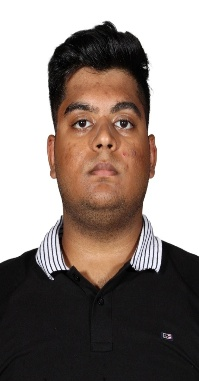
\includegraphics[width=1in,height=1.25in,clip,keepaspectratio]{photo1.jpg}}]{Syed Ayman Alam}
was born in Bengaluru, India, in 2005, and is pursuing the B.Tech. degree in computer science and engineering (AI \& ML) at Vellore Institute of Technology (VIT), Vellore, India, School of Computer Science and Engineering (SCOPE).
\end{IEEEbiography}
\begin{IEEEbiography}[{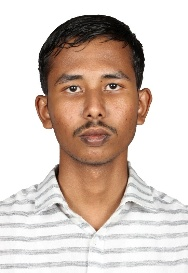
\includegraphics[width=1in,height=1.25in,clip,keepaspectratio]{photo2.jpg}}]{Girijeshvasan M}
was born in Tamil Nadu, India, in 2006, and is pursuing the B.Tech. degree in computer science and engineering at Vellore Institute of Technology (VIT), Vellore, India, School of Computer Science and Engineering (SCOPE).
\end{IEEEbiography}
\begin{IEEEbiography}[{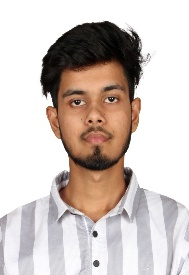
\includegraphics[width=1in,height=1.25in,clip,keepaspectratio]{photo3.jpg}}]{Brajesh Agrawal}
was born in Bihar, India, in 2004, and is pursuing the B.Tech. degree in computer science and engineering at Vellore Institute of Technology (VIT), Vellore, India, School of Computer Science and Engineering (SCOPE).
\end{IEEEbiography}

\end{document}
